% =========================================================================== %
% Introduction
% =========================================================================== %

\ifx\wholebook\relax\else
  \documentclass[a4paper,10pt,twoside]{book}
  %=============================================================================%
% Common things, settings, packages to include
%=============================================================================%

\usepackage{graphicx}
\usepackage{color}
\usepackage{makeidx}
\usepackage{ifpdf}
\usepackage{verbatim}

% --------------------------------------------------------------------------- %
% Setting up stuff depeding on output format
% --------------------------------------------------------------------------- %

\ifpdf
  % special settings for pdf mode
  \usepackage[colorlinks]{hyperref}
  \usepackage{courier}
  
  \hypersetup{
    colorlinks,
    linkcolor=darkblue,
    citecolor=darkblue,
    pdftitle={The Eclipse Scout Book},
    pdfauthor={The Scout Community},
    pdfkeywords={Enterprise Framework, Eclipse, Java, Client-Side, Rich Client, Web Client, Mobile},
    pdfsubject={Computer Science}
  }
  
  \usepackage{caption}
  \captionsetup{margin=10pt,font=small,labelfont=bf}
\else
  % special stuff for html mode
  \usepackage[tex4ht]{hyperref}
\fi

% --------------------------------------------------------------------------- %
% Setting up printing range
% --------------------------------------------------------------------------- %

\parindent 1cm
\parskip 0.2cm
\topmargin 0.2cm
\oddsidemargin 1cm
\evensidemargin 0.5cm
\textwidth 15cm
\textheight 21cm

% --------------------------------------------------------------------------- %
% Setting up listings
% --------------------------------------------------------------------------- %

\usepackage{listings}
 
\definecolor{darkviolet}{rgb}{0.5,0,0.4}
\definecolor{darkgreen}{rgb}{0,0.4,0.2} 
\definecolor{darkblue}{rgb}{0.1,0.1,0.9}
\definecolor{darkgrey}{rgb}{0.5,0.5,0.5}
\definecolor{lightblue}{rgb}{0.4,0.4,1}
\definecolor{lightgray}{rgb}{0.97,0.97,0.97}

\renewcommand{\lstlistlistingname}{List of Listings}

% general settings
\lstset{
  basicstyle=\small\ttfamily,
  columns=fullflexible,
  breaklines=true,
  breakindent=10pt,
  prebreak=\mbox{{\color{blue}\tiny$\searrow$}},
  postbreak=\mbox{{\color{blue}\tiny$\rightarrow$}},
  showstringspaces=false,
  backgroundcolor=\color{lightgray}
}

% settings for xml files
\lstdefinelanguage{xml}
{
  commentstyle=\color{darkgrey}\upshape,
  morestring=[b]",
  morestring=[s]{>}{<},
  morecomment=[s]{<?}{?>},
  stringstyle=\color{black},
  identifierstyle=\color{darkblue},
  keywordstyle=\color{cyan},
  morekeywords={xmlns,name,point,factory,class}% list your attributes here
}

% settings for ini files
\lstdefinelanguage{ini}
{
  morecomment=[f][\color{darkgrey}\upshape][0]\#, % # is comment iff it's the first char on the line
  stringstyle=\color{black}
}

% default settings (for java files)
\lstset{
  language=Java,
  emphstyle=\color{red}\bfseries,
  keywordstyle=\color{darkviolet}\bfseries,
  commentstyle=\color{darkgreen},
  morecomment=[s][\color{lightblue}]{/**}{*/},
  stringstyle=\color{darkblue},
}

% --------------------------------------------------------------------------- %
% cross reference macros
% --------------------------------------------------------------------------- %
\newcommand{\applabel}[1]{\label{apx:#1}}
\newcommand{\chalabel}[1]{\label{cha:#1}}
\newcommand{\seclabel}[1]{\label{sec:#1}}
\newcommand{\lstlabel}[1]{\label{lst:#1}}
\newcommand{\figlabel}[1]{\label{fig:#1}}
\newcommand{\tablabel}[1]{\label{tab:#1}}

\newcommand{\appref}[1]{Appendix~\ref{apx:#1}}
\newcommand{\charef}[1]{Chapter~\ref{cha:#1}\xspace}
\newcommand{\secref}[1]{Section~\ref{sec:#1}}
\newcommand{\lstref}[1]{Listing~\ref{lst:#1}\xspace}
\newcommand{\figref}[1]{Figure~\ref{fig:#1}\xspace}
\newcommand{\tabref}[1]{Table~\ref{tab:#1}\xspace}

% --------------------------------------------------------------------------- %
% graphics paths
% --------------------------------------------------------------------------- %
\graphicspath{
  {figures/}
  {Introduction/figures/}
}

%=============================================================================%

  \pagestyle{headings}
  \graphicspath{{figures/} {../figures/} {../modules/figures/}}
  \begin{document}
  \sloppy
\fi


% =========================================================================== %
\chapter{Introduction}

% --------------------------------------------------------------------------- %
\section{What is Scout?}
\seclabel{what_is_scout}

Scout is an open source framework for building business applications.
The Scout framework covers most recurring aspects of a classical client server architecture with a strong focus on the application's front-end. 
With its multi-device capability, a Scout client applications may run simultaneously as a rich client, in the browser and on mobile and tablet devices. 

To different groups of people, Scout means different things. 
End users are interested in a good usability, the management cares about the benefits a new framework can offers to the organisation and developers want to know if a framework is simple to use and helps them to solve practical issues. 
This is why the text below describes Scout from the perspective of these three roles.

% ........................................................................... %
\subsection{End User Perspective}

End users of enterprise applications care about friendly user interfaces (UI) and well designed functionality that support them in their everyday work. 
Depending on the current context/location of an end user, either desktop, web or mobile clients work best. 
If working in the office, a good integration of the enterprise software with Lotus Notes or Microsoft Office often help to boost the users productivity. 
As office software is typically installed locally on the users PC, integrating this software also requires a desktop client for the enterprise application. 
When a user is working on a computer outside of his company where the enterprise client is not installed (or the user lacks the permissions to install any software), the natural choice is to work with a web application.
And when the user is on the move or sitting in a meeting, the only meaningful option is to work with a mobile device. 

\begin{figure}
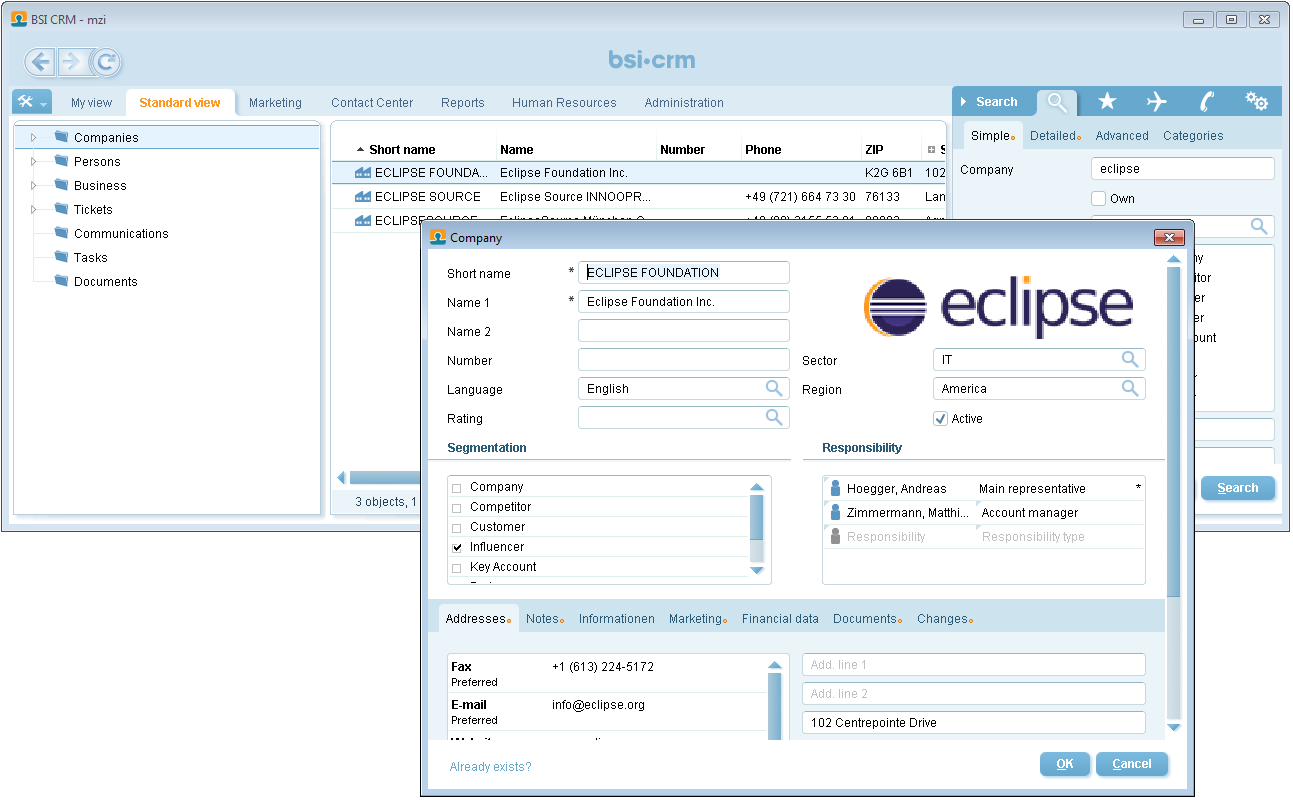
\includegraphics[width=14cm]{bsi_crm_desktop.png}
\caption{The desktop client of a Scout enterprise application.}
\figlabel{bsi_crm_desktop}
\end{figure}

To provide a concrete example, we briefly describe a real world enterprise application based on Scout. 
A first screenshot of a Scout desktop client is provided in \figref{bsi_crm_desktop}. 
The screenshot provides an overview of the layout of a customer relationship management (CRM) solution. 
On the left hand side, an entity class such as companies can be selected. 
Once an entity such is selected, a form is presented on the right hand side to enter the search criteria.
After entering ''eclipse'' into the company search field, the list of matching companies is presented.
Using the context menu on a specific company, the corresponding company dialog can be opened for editing.

\begin{figure}
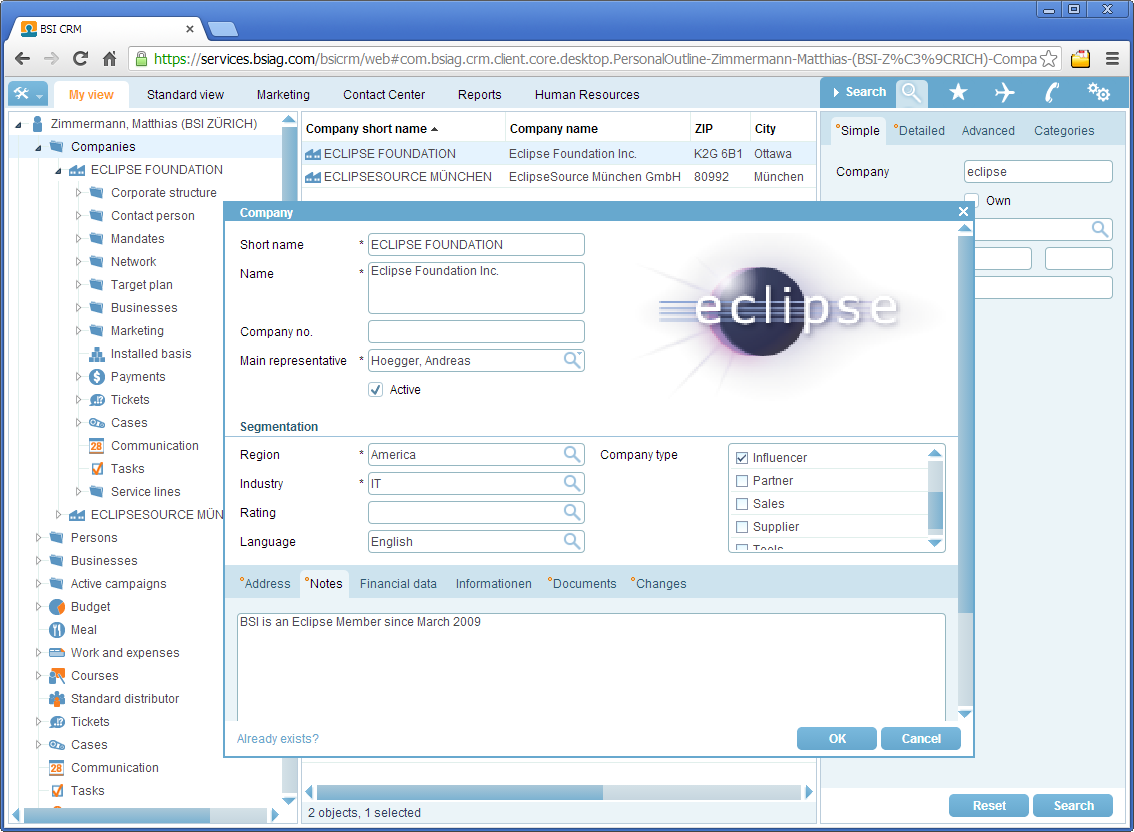
\includegraphics[width=14cm]{bsi_crm_web.png}
\caption{A Scout enterprise application running in a web browser.}
\figlabel{bsi_crm_web}
\end{figure}

In \figref{bsi_crm_web} a screenshot of the web client of the CRM Scout application is shown. 
When comparing the screenshots of the desktop client with the web application it is interesting to note how Scout applications offer a consistent look and feel for the two clients. 
This is important as it makes the end user feel ''at home'' on the web client. 

\begin{figure}
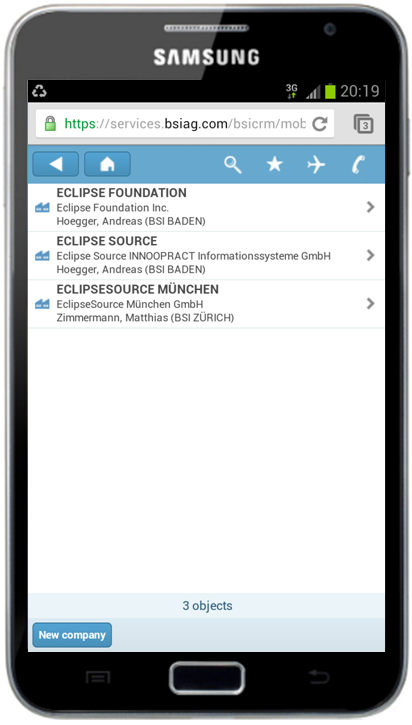
\includegraphics[width=7cm]{bsi_crm_mobile_galaxy.png}
\caption{The same Scout enterprise application running on a mobile device.}
\figlabel{bsi_crm_mobile}
\end{figure}

Finally, \figref{bsi_crm_mobile} provides a screenshot of the now familiar CRM application. 
In contrast to desktop and web applications, most tablets and mobile phones are controlled using touch features instead of mouse clicks.
In addition, less elements may be presented on a single screen compared to desktop devices.
These two aspects makes it impractical to directly reuse the desktop user interface on mobile devices.
The look and feel still relates to the desktop and web clients but is optimized to the different form factor of the mobile device. 
And the end user benefits from the identical behaviour and the the known functionality of the application.

Comparing the company table shown in the background of \figref{bsi_crm_desktop} with \figref{bsi_crm_mobile} it can be observed that the multi-column table of the desktop client has been transformed into a list on the mobile device. 
In addition, the context menu ''New company'' is now provided as a touch button.
As the navigation in the application and the offered choices remain the same for Scout desktop and mobile applications, the end user feels immediately comfortable working with Scout mobile applications.

% ........................................................................... %
\subsection{Management Perspective}

For the management, Scout is best explained in terms of benefits it brings to the organisation in question. 
This is why we are going to concentrate on a (typical) application migration scenario here. 
Let us assume that to support the company's business, a fairly large landscape of multi-tier applications has to be maintained and developed. 
Including host systems, client server applications with desktop clients, as well as applications with a web based front-end. 

\begin{figure}
\includediagram{14cm}{scout_with_other_apps}
\caption{A typical application landscape including a service bus and a Scout application.}
\figlabel{scout_with_other_apps}
\end{figure}

Usually, these applications interact with each other through a service bus as shown in \figref{scout_with_other_apps}. 
Often, some of the applications that are vital to the organisation's core business have grown historically and are based on legacy technologies. 
And for technologies that are no longer under active development it can get difficult to find staff having the necessary expertise or motivation. 
Sometimes, the organisation is no longer willing to accept the costs and technology risks of such mission critical applications. 

\begin{figure}
\includediagram{14cm}{scout_integration}
\caption{The integration of a Scout application in a typical enterprise setup.}
\figlabel{scout_integration}
\end{figure}

In this situation, the company needs to evaluate if it should buy a new standard product or if the old application has to be migrated to a new technology stack. 
Now let us assume, that available products do not fit the company's requirements well enough and we have to settle for the migration scenario.
In the target architecture, a clean layering similar to the one shown in \figref{scout_integration} is often desirable.

While a number of modern and established technologies exist that address the backend side (data bases, data access and business services), the situation is different for the UI layer and the application layer. 
The number of frameworks to develop web applications with Java is excessively large\footnote{
Web application framework comparison: \url{http://en.wikipedia.org/wiki/Comparison_of_web_application_frameworks#Java}.
},
but the choice between desktop application technologies in the Java domain is restricted to three options only. 
Swing, SWT and JavaFX.
Both Eclipse SWT and Java Swing are mature and well established but Swing is moving into 'maintenance only' mode and will be replaced by JavaFX.
However, the maturity of the new JavaFX technology in large complex enterprise applications is not yet established. 
Obviously, deciding for the right UI technology is a challenge and needs to be made very carefully. 
Reverting this decision late in a project or after going into production can get very expensive and time consuming. 

Once the organisation has decided for a specific UI technology, additional components and frameworks need to be evaluated to cover client server communication, requirements for the application layer, and integration into the existing application landscape. 
To avoid drowning in the integration effort for all the elements necessary to cover the UI and the application layer a 'lightweight' framework is frequently developed. 
When available, this framework initially leads to desirable gains in productivity. 
Unfortunately, such frameworks often become legacy by themselves. 
Setting up a dedicated team to actively maintain the framework and adapt to new technologies can reduce this risk. 
But then again, such a strategy is expensive and developing business application frameworks is usually not the core business of a company. 

Can we do better? 
To implement a business application that covers the UI and the application layer as shown in \figref{scout_integration}, Eclipse Scout substantially reduces both risk and costs compared to the inhouse development presented above.
First or all, Scout is completely based on Java and Eclipse. 
Chances are, that developers are already familiar with some of these technologies.
This helps in getting developers up to speed and keeping training costs low. 

On the UI side, Scout's multi-device support almost allows to skip the decision for a specific UI technology. 
Should a particular web framework become the de-facto standard in the next years, it will be the responsibility of the Scout framework to provide the necessary support. 
Existing Scout applications can then switch to this new technology with only minimal effort. 
This is possible because the Scout developers are designing and building the UI of an application using Scout's client model.
And this client model is not linked to any specific UI technology. 
Rather, specific UI renderers provided by the Scout framework are responsible to draw the UI at runtime. 

As Scout is an open source project, no licence fees are collected. 
Taking advantage of the growing popularity of Scout, free community support is available via a dedicated forum. 
At the same time, professional support is available if the organisation decides for it.

As the migration of aging applications to current technology is always a challenge, it surely helps to have Scout in the technology portfolio. 
Not only is it a low risk choice, but also boosts developer productivity and helps to motivate the development team. 
Additional reasons on why Scout helps to drive down cost and risks are discussed in \secref{why_scout}.

% ........................................................................... %
\subsection{Developer Perspective}

From the perspective of application developers, Scout offers a Java based framework that covers the complete client server architecture. 
This implies that -- once familiar with the Scout framework -- the developer can concentrate on a single framework language (Java) and a single set of development tools. 

As Scout is completely based on Java and Eclipse, Scout developers can take full advantage of existing knowledge and experience in these domains. 
And to make learning Scout as simple as possible, Scout includes a comprehensive software development kit (SDK), the Scout SDK.
The Scout SDK helps to create a robust initial project setup for client server applications and includes a large set of wizards for repetitive and error prone tasks.

On the client-side Scout's flexible client model allows the developer to create a good user experience without having to care about specific UI technologies. 
The reason for this can be found in Scout's client architecture that cleanly separates the UI model from the UI technology.
In Scout (almost) every UI component is implemented four times. 
First the implementation of the UI model component and then, three rendering components for each UI technology supported by Scout. 
For desktop clients these are the Swing and the SWT technologies, and for the web and mobile support this is Eclipse RAP which in turn takes care of the necessary JavaScript parts.  

Not having to worry about Swing, SWT or JavaScript can significantly boost the productivity.
With one exception. 
If a specific UI widget is missing for the user story to be implemented, the Scout developer first needs to implement such a widget. 
Initially, this task is slightly more complex than not working with Scout. 
For custom widgets the Scout developer needs to implement both a model component and a rendering component for a specific UI technology. 
But as soon as the client application needs to be available on more than a single frontend, the investment already pays off.
The developer already did implement the model component and only needs to provide an additional rendering component for the new UI technology.
In most situations the large set of Scouts UI components provided out-of-the box are sufficient and user friendly applications are straight forward to implement. 
Even if the application needs to run on different target devices simultaneously.

Client-server communication is an additional aspect where the developers is supported by Scout.
Calling remote services in the client application that are provided by the Scout server looks identical to the invocation of local services. 
The complete communication including the transfer of parameter objects is handled fully transparent by the Scout framework.
In addition, the Scout SDK can completely manage the necessary transfer objects to fetch data from the Scout server that is to be shown in dialog forms on the Scout client.
The binding of the transferred data to the form fields is done by the framework.

Although the Scout SDK wizards can generate a significant amount of code, there is no one-way code generation and no meta data in a Scout application.
Just the Java code\footnote{
With the exception of the \filename{plugin.xml} and \filename{MANIFEST.MF} files required for Eclipse plugins.
}. 
Developers preferring to write the necessary code manually, may do so. 
The Scout SDK parses the application's Java code in the background to present the updated Scout application model to the developers preferring to work with the Scout SDK. 

Finally, Scout is an open source framework hosted at the Eclipse foundation. 
This provides a number of interesting options to developers that are not available for closed source frameworks. 
First of all, it is simple to get all the source code of Scout and the underlying Eclipse platform. 
This allows for complete debugging of all problems and errors found in Scout applications. 
Starting from the application code, including the Scout framework, Eclipse and down to the Java platform. 

Scout developer can also profit from an increasing amount of free and publicly available documentation, such as this book or the Scout Wiki pages. 
And problems with Scout or questions that are not clearly addressed by existing documentation can be discussed in the Scout forum. 
The forum is also a great place for Scout developers to help out in tricky situation and learn from others. 
Ideally, answered questions lead to improved or additional documentation in the Scout Wiki.

At times, framework bugs can be identified from questions asked in the forum. 
As all other enhancement requests and issues, such bugs can be reported in Bugzilla by the Scout developer. 
Using Bugzilla, Scout developers can also contribute bug analysis and patch proposals to solve the reported issue.
With this process, Scout developers can actively contribute to the code base of Eclipse Scout.
This has the advantage, that workarounds in existing Scout applications can be removed when an upgrade of the Scout framework is made.

Having provided a significant number of high quality patches and a meaningful involvement in the Scout community, the Scout project can nominate a Scout developer as a new Scout committer. 
Fundamentally, such a nomination is based on the trust of Scout committers in the candidate. 
To quote the official guidelines\footnote{
Nominating and electing a new Eclipse Scout committer: \url{http://wiki.eclipse.org/Development_Resources/HOWTO/Nominating_and_Electing_a_New_Committer#Guidelines_for_Nominating_and_Electing_a_New_Committer}.
} 
for nominating and electing a new committer:

\begin{quotation}
\begin{em}
\htmlit
A Committer gains voting rights allowing them to affect the future of the Project. 
Becoming a Committer is a privilege that is earned by contributing and showing discipline and good judgment. 
It is a responsibility that should be neither given nor taken lightly, nor is it a right based on employment by an Eclipse Member company or any company employing existing committers.
\htmlitend
\end{em}
\end{quotation}

\noindent After a successful election process (existing committers voting for and not against the candidate) the Scout developer effectively becomes a Scout committer. 
With this new status, the Scout developer then gets write access to the Eclipse Scout repositories and gains voting rights and the possibility to shape the future of Scout. 

% --------------------------------------------------------------------------- %
\section{Why Scout?}
\seclabel{why_scout}

Most large organizations develop and maintain enterprise applications that have a direct impact on the success of the ongoing business. 
And at the same time, those responsible for the development and maintenance of these applications struggle with this task. 
It is a big challenge to adapt to changing business demands and complying with the latest legal requirements in time. 
And the increasing pressure to lower recurring maintenance costs does not make the situation any easier.

It often seems that too many resources are required to keep a heterogeneous set of legacy technologies alive. 
In this situation, modernizing mission critical applications can help to improve over the current situation. 
For the target platform stack, Java is a natural choice as it is mature, widely adopted by in the industries and unlikely to become legacy in the foreseeable future. 
While for the back-end side of enterprise applications well-known and proven frameworks do exist, the situation on the client side is less clear. 
Unfortunately, user interface (UI) technologies often have lifetimes that are substantially shorter than the lifetimes of larger mission critical applications. 
This is particularly true for the web, where many of today's frameworks will no longer be relevant in five or more years. 

Enter Eclipse Scout. This open source framework covers most of the recurring needs that are relevant to the front-end development of business applications. 
And Scout forces a clean separation between the user interface and the specific UI technology used for rendering. 
This has two major benefits. 
First, Scout developers implement the user interface against an abstraction layer, which helps to focus on the business functionality and saves development time. 
And second, long term maintenance costs are lower, as the Scout code remains valid even when the rendering technology needs to be exchanged. 
Therefore, Scout helps to improve the productivity of the development teams and reduces the risk of major application rewrites. 

To provide a first impression on the scope and goals of the Scout framework, a number of scenarios where Scout typically contributes to your projects success are listed below . 

\begin{itemize}
\item You are looking for a reasonable client side framework for your business application.  
\item You need an application that works on the desktop, in browsers and on mobiles devices. 
\item You don't have the time to evaluate and learn a new UI technology. 
\item You need a working prototype application by the end of the week. 
\item Your application's expected lifespan is 10 years or more. 
\end{itemize}

\noindent That Scout should help in the last two situations mentioned above seems to be contradictory at first but is just based on a simple principle.  
Where possible, the Scout framework provides abstractions for areas/topics\footnote{
Example areas/topics that are abstracted by the Scout framework are user interface (UI) technologies, databases, client-server communication or logging. 
} 
that need to be implemented for business applications again and again. 
And for each of these abstractions Scout provides a default implementation out of the box.
Typically, the default implementation of such an abstraction integrates a framework or technology that is commonly used. 

When needing a working prototype application by the end of the week, the developer just needs to care about the desired functionality. 
The necessary default implementations are then automatically included by the Scout tooling into the Scout project setup.
The provided Scout SDK tooling also helps to get started quickly with Scout. 
It also allows to efficiently implement application components such as user interface components, server services or connections to databases.

In the case of applications with long lifespans, the abstractions provided by Scout help the developer to stay productive and concentrate on the actual business functionality. 
At the same time, this keeps the code base as independent of specific technologies and frameworks as possible. 
This is a big advantage when individual technologies incorporated in the application reach their end of life. 
As all the implemented business functionality is written against abstractions only, no big rewrite of the application is necessary. 
Instead, it is sufficient to exchange the implementation for the legacy technology with a new one. 
And often, an implementation for a new technology/framework is already provided by a more recent version of Scout. 

% --------------------------------------------------------------------------- %
\section{What should I read?} 
\seclabel{whatshouldiread}

The text below provides guidelines on what to read (or what to skip) depending on your existing background.
We first address the needs of junior Java developers that like to learn more about developing enterprise applications.
Then, we suggest a list of sections relevant for software wizards that already have a solid understanding of the Eclipse platform, Java enterprise technologies, and real world applications.
Finally, the information needs of IT managers are considered.

% ........................................................................... %
\subsection{I know Java}

The good news first.
This book is written for you! 
For the purpose of this book we do not assume any significant understanding of the Java Enterprise Edition (Java EE)\footnote{
Java Enterprise Edition: \url{http://en.wikipedia.org/wiki/Java_Platform,_Enterprise_Edition}
}
and the Eclipse Platform\footnote{
Eclipse Platform: \url{http://wiki.eclipse.org/Platform}
}. 

Of course, having prior experience in client server programming with Java is helpful.
And having used the Eclipse IDE for Java development before --- please do not mistake the IDE with the Eclipse platform\footnote{
By reading through the book you will learn that there is much more to the Eclipse platform than just the IDE
}
is certainly of benefit.

The ``bad'' news is, that writing Scout applications requires a solid understanding of Java.
To properly benefit from this book, we assume that you have been developing software for a year or more.
And you should have mastered the Java Standard Edition 
(Java SE)\footnote{
Java Standard Edition: \url{http://en.wikipedia.org/wiki/Java_SE}
} 
to a significant extent. 
To be more explicit, you are expected to be comfortable with all material required for the Java Programmer Level I 
Exam\footnote{
Level I Exam: \url{docs.oracle.com/javase/tutorial/extra/certification/javase-7-programmer1.html}
}
and most of the material required for 
Level II\footnote{
Level II Exam: \url{docs.oracle.com/javase/tutorial/extra/certification/javase-7-programmer2.html}
}.

We now propose to start downloading and installing Scout as described in \appref{install_scout} and do some actual coding.
To do so, please continue with the ``Hello World'' example provided in \charef{helloworld}.
You can expect to complete this example in less than one hour including the necessary download and installation steps.
Afterwards, you might want to continue with the remaining material in ``Getting Started''. 
Working through the complete book should take no more than two days. 

Once you work with the Scout framework on a regular basis, you might want to ask questions in the Scout 
forum\footnote{
Eclipse Scout forum: \url{http://www.eclipse.org/forums/eclipse.scout}
}.
When your question gets answered, please ask yourself if your initial problem could have been solved by better documentation.
In that case, you might want to help the Scout community by fixing or amending the Scout wiki pages\footnote{
Eclipse Scout wiki: \url{http://wiki.eclipse.org/Scout}
}.
Or this book. 
If you find a bug in Eclipse Scout that makes your life miserable you can report it or even propose a patch. 
And when your bug is fixed, you can test the fix.
All of these actions will add to the healthy grow of the Scout community.

% ........................................................................... %
\subsection{I know tons of both Java and Eclipse}

This means that you are one of these software wizards that get easily bored.
You prefer to get a quick impression before deciding to dig deeper and hate going through lengthy descriptions.
In that case let us assume that you are prepared to spend two hours to grasp the scope of Eclipse Scout and get an impression of its strengths and limitations.
The list below suggests a sequence of sections to digest including a brief motivation for each one.

\begin{itemize}
  \item \charef{helloworld} ''Hello World'' Tutorial. 
      Download and installation of the Scout package should take less than 30 minutes, going through the ''Hello World'' takes another 15 minutes. 
  \item \secref{initial_helloworld} ``Walking through the Initial Application''
      Read about some key elements used in every Scout client application including integration of server services and data binding.
  \item \charef{tooling} ``Scout Tooling''.
      Browse through the tooling chapter to get an impression on the tooling provided with Scout. 
	  Make sure you understand that the Scout SDK is supporting the developer without restricting the developer.
  \item \charef{large_example} ``The My Contacts Application''. 
      Check out the slightly larger demo application. 
	  In case you are not yet running out of time, download the demo app as described in the Scout wiki\footnote{
		Download and installation of the ''My Contacts'' application: \url{http://wiki.eclipse.org/Scout/Book/\#Download_and_Run_the_Scout_Sample_Applications}.
	  }.
\end{itemize}

% ........................................................................... %
\subsection{I am a manager}

Being a manager and actually reading this book may indicate one of the following situations:

\begin{itemize}
  \item Your developer tried to convince you that Eclipse Scout can help you with implementing business applications in a shorter time and for less money.
        And you did not understand why (again) a new technology should work better than the ones you already use. 
  \item Your are a product manager of a valuable product that is based on legacy technology. 
        And you are now evaluating options to modernize your product.
  \item Think about your current situation. There must be a reason why you are checking out this book.
\end{itemize}

To learn about Scout and about its benefits first go through \secref{what_is_scout} and \secref{why_scout}.
Then, flip through \secref{my_contacts_guide} to get an impression of the ''My Contacts'' application. 
In case you like the idea that your developers should be able to build such an application in a single day, you might want to talk to us\footnote{
To contact the Scout team, use the feedback provided on the Scout homepage: \url{https://eclipse.org/scout}.
}.


% =========================================================================== %
\chapter{''Hello World'' Tutorial}
\chalabel{helloworld}

The ''Hello World'' chapter walks you through the creation of an Eclipse Scout client server application.
When the user starts the client part of this application, the client connects to the server\footnote{
The Scout server part of the ''Hello World'' application will be running on a web server.
} 
and asks for some text content that is to be displayed to the user.
Next, the server retrieves the desired information and sends it back to the client.
The client then copies the content obtained from the server into a text field widget.
Finally, the client displays the message obtained from the server in a text field widget.

The goal of this chapter is to provide a first impression of working with the Scout framework using the Scout SDK.
We will start by building the application from scratch and then we'll deploy the complete application to a Tomcat web server.
Except for a single line of code in the server part of the ''Hello World'' application, we will only be using the tooling provided by the Scout SDK.

Based on this simple ''Hello World'' applications a large number of Scout concepts can be illustrated.
Rather than including such background material in this tutorial, this information is provided separately in \charef{helloworld_background}.
This tutorial is also available in the Scout wiki\footnote{
''Hello World'' wiki tutorial: \url{http://wiki.eclipse.org/Scout/Tutorial/4.0/HelloWorld}
}.

% --------------------------------------------------------------------------- %
\section{Installation and Setup}

Before you can start with the ''Hello World'' example you need to have a complete and working Scout installation.
For this, see the step-by-step installation guide provided in \appref{install_scout}.
Once you have everything installed, you are ready to create your first Scout project.

% --------------------------------------------------------------------------- %
\htmlanchor{create_project_simple}
\section{Create a new Project}
\seclabel{create_project_simple}
\index{Project creation}

% =========================================================================== %
% TeX input file: "Create a new project"
%
% WARNING: this tex file does not compile standalone, it needs to be embedded
% in a master tex document (e.g. Introduction.tex)
% =========================================================================== %

Start your Eclipse IDE and select an empty directory for your workspace. 
This workspace directory will then hold all the project code for the ''Hello World'' application. 
Once the Eclipse IDE is running it will show the Scout perspective with the ''Scout Explorer'' view and an empty ''Scout Object Properties'' view.
To create a new Scout project select the \contextmenu{New Scout Project...} as shown in \figref{sdk_create_new_scout_project}.

\begin{figure}
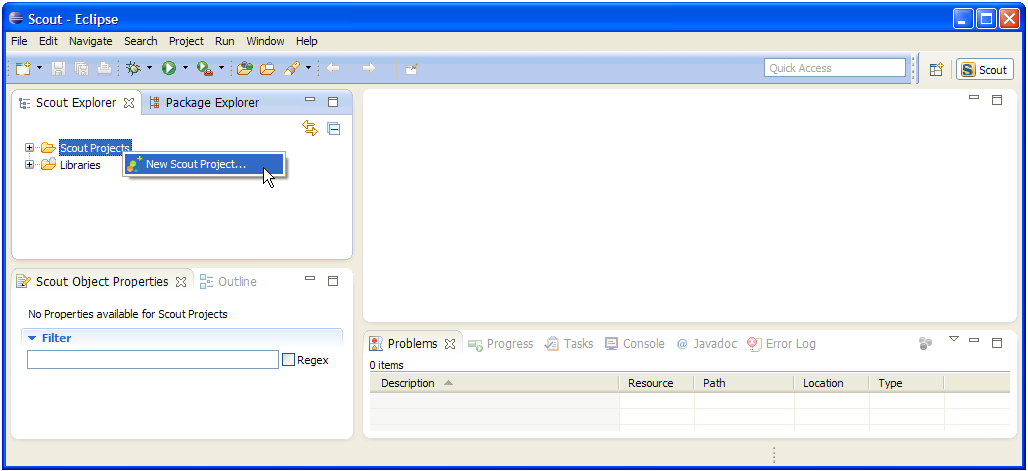
\includegraphics[width=15cm]{sdk_create_new_scout_project.png}
\caption{Create a new Scout project using the Scout SDK perspective.}
\figlabel{sdk_create_new_scout_project}
\end{figure}

In the \wizard{New Scout Project} enter a name for your Scout project. 
As we are creating a ''Hello World'' application, use \java{org.eclipsescout.helloworld} for the \field{Project Name} according to \figref{sdk_new_project_wizard}.
Then, click the \button{Finish} to let the Scout SDK create the initial project code for you.

\begin{figure}
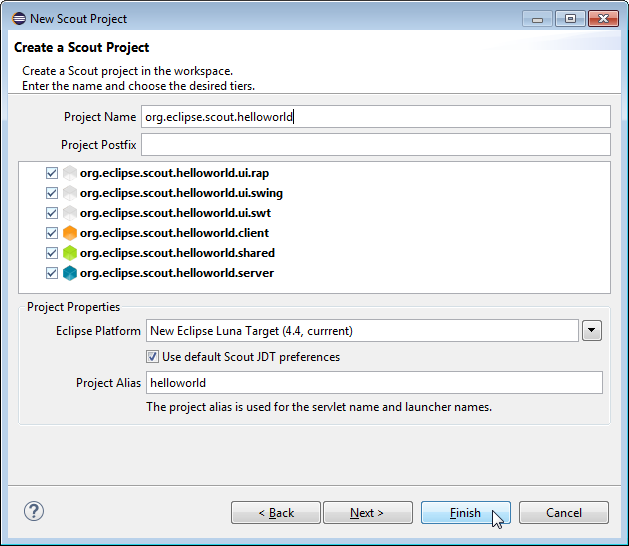
\includegraphics[width=6cm]{sdk_new_project_2.png}
\caption{The new Scout project wizard.}
\index{SDK Wizard!New Scout Project}
\figlabel{sdk_new_project_wizard}
\end{figure}

Once the initial project code is built, the Scout SDK displays the application model in the \textit{Scout Explorer} as shown in \figref{sdk_initial_helloworld_project}.
This model is visually presented as a tree structure covering both the client and the server part of the application.
The Scout Explorer view on the left hand side displays the top level elements of the complete Scout application.
Under the orange node the Scout client components are listed. 
Components that are needed in both the Scout client and the Scout server are collected under the green node.
And the Scout server components are listed below the blue node in the Scout Explorer view.

\begin{figure}
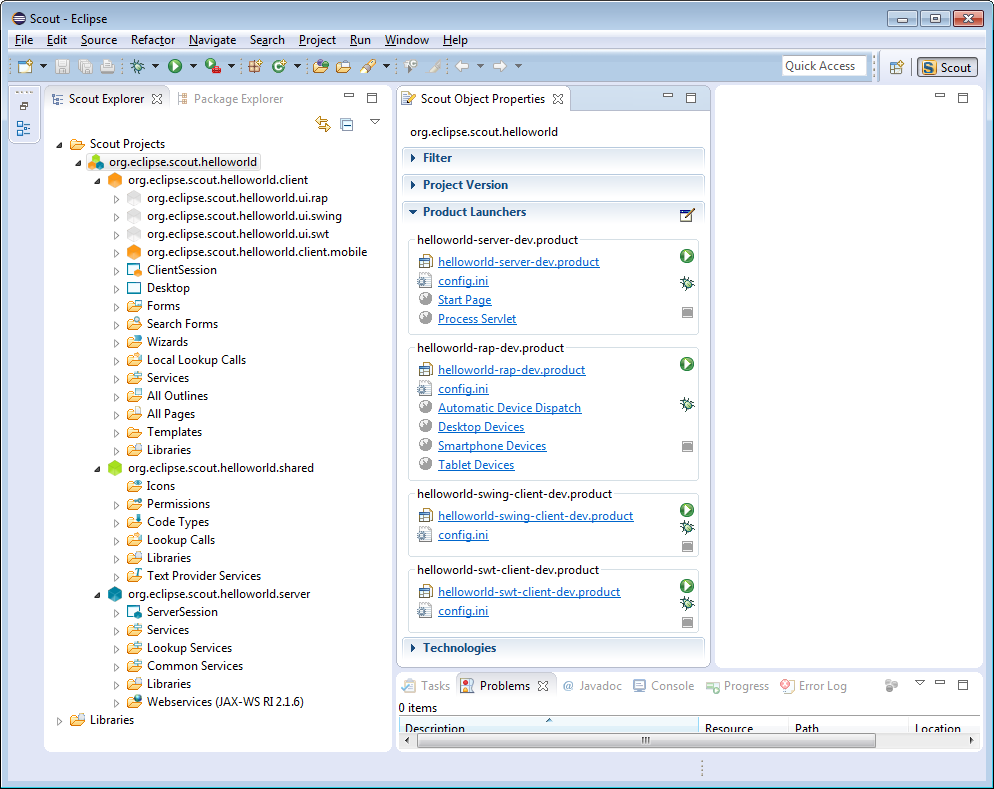
\includegraphics[width=15cm]{sdk_initial_helloworld_project.png}
\caption{The Scout SDK showing the tree representation of our ''Hello World'' application in the Scout Explorer.
The Scout Object Properties contain the product launchers for the server and the available clients.}
\figlabel{sdk_initial_helloworld_project}
\end{figure}

% =========================================================================== %
% EOF TeX input file
% =========================================================================== %


% --------------------------------------------------------------------------- %
\section{Run the Initial Application}
\seclabel{run_initial}

After the initial project creation step we are ready to start the server and the clients of the still empty Scout application.
For this, we switch to the Scout Explorer and select the root node \element{org.eclipse.scout.helloworld}.
Selecting the application's \node{org.eclipse.scout.helloworld} in the Scout Explorer displays the product launchers in the \textit{Scout Object Properties}.
As we can see in \figref{start_client}, we have product launchers for four different development products.

\begin{tabular}{ l l }
  \textbf{Server} & The Scout server application\\
  \textbf{RAP}    & The RAP server application for web and mobile clients\\
  \textbf{Swing}  & The Scout Swing desktop client application\\
  \textbf{SWT}    & The Scout SWT desktop client application\\
\end{tabular}

\begin{figure}
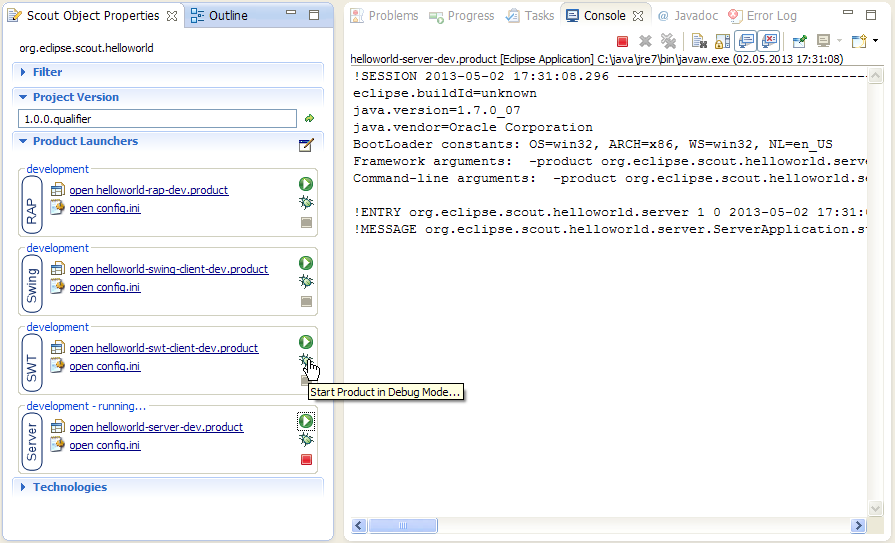
\includegraphics[width=15cm]{sdk_start_client_product.png} 
\caption{Starting the web client in the Scout SDK using the provided RAP product launcher. Make sure to start the server before starting any client product.}
\figlabel{start_client}
\index{Product launchers}
\end{figure}

Each product launcher box provides a link to the corresponding Eclipse product file\footnote{
Product files define the set of all components that are necessary to build the complete application.
},
the configuration file\footnote{
The configuration file \filename{config.ini} provides parameters that are read at startup of the corresponding program.
},
as well as three launcher icons to start and stop the corresponding application.
The green \icon{Circle} starts the product in normal mode.
The \icon{Bug} just below, starts a product in debug mode.
To terminate a running product, the red \icon{Square} is provided. 
Alternatively, you can also stop products by clicking on the same red icon in the console view.
This is shown on the right hand side of \figref{start_client}.
Client products may also be stopped by closing the client's main window or using the provided \menu{File|Exit}.

Before any of the client products is started, we need to start the server product using the green circle or the bug launcher icon.
During startup of the Scout server you should see console output similar to the one shown on the right hand side of \figref{start_client}.
Once the server is running, you may start the web client as shown in \figref{start_client}, the Swing client, or the SWT client in the same way.
And with a running RAP product, the Scout web client can be opened in a web browser.
Just click on the provided \link{Automatic Device Dispatch} or open a a browser and manually type the address \texttt{http://localhost:8082/web} into the browser's navigation bar.

\begin{figure}
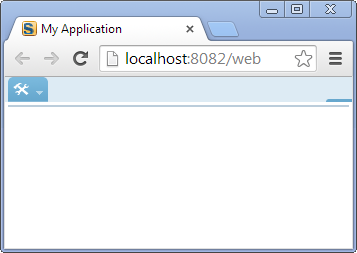
\includegraphics[width=4.5cm]{hellworld_empty_rap.png} \hspace{3mm}
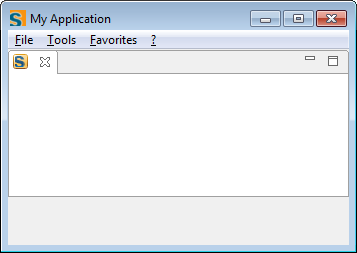
\includegraphics[width=4.5cm]{hellworld_empty_swing.png} \hspace{3mm}
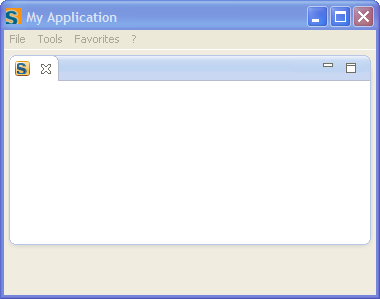
\includegraphics[width=4.5cm]{hellworld_empty_swt.png}
\caption{Running the three client applications. 
Each client displays an empty desktop form. 
From left to right: The web client, the Swing client, and the SWT client}
\figlabel{helloworld_empty}
\end{figure}

Having started the Scout server and all client products, the client applications should become visible as shown in \figref{helloworld_empty}.

% --------------------------------------------------------------------------- %
\section{The User Interface Part}
\seclabel{helloworld_ui}

% =========================================================================== %
% TeX input file: "Create the hello world frontend"
%
% WARNING: this tex file does not compile standalone, it needs to be embedded
% in a master tex document (e.g. Introduction.tex)
% =========================================================================== %

The project creation step has created a Scout client that displays an empty desktop form.
We will now add widgets to the client's desktop form that will later display the ''Hello World!'' message.

To add any widgets to the desktop form, we first need to navigate to the \element{DesktopForm} in the Scout Explorer.
For this, first navigate to the orange client node in the Scout Explorer view.
Then, expand the \element{Forms} folder by clicking on the small triangle icon, and further expand the \element{DesktopForm}. 
As a result, the \element{MainBox} element becomes visible below the desktop form as shown in \figref{new_field_context_menu}. 
With a click of the right mouse button over the \element{MainBox}, the available context menus are displayed.
To start the form field wizard we select the \menu{New Form Field ...}.

\begin{figure}
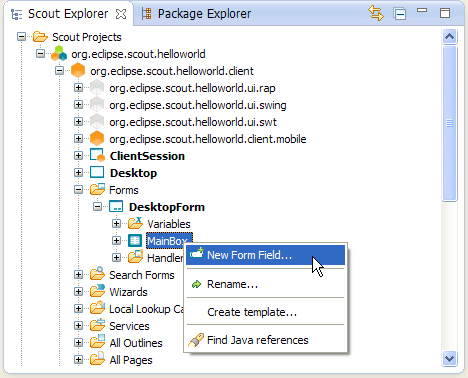
\includegraphics[width=8cm]{sdk_new_field_wizard_menu.png} 
\caption{Using the \menu{New Form Field ...} to start the form field wizard provided by the Scout SDK.}
\figlabel{new_field_context_menu}
\end{figure}

In the first step of the form field wizard shown on in \figref{helloworld_groupboxfield} we choose \java{GroupBox} as the form field type and click on the \button{Next}.
In the second wizard step, we enter 'Desktop' into the \field{Class Name} before we close the wizard with the \button{Finish}.
The Scout SDK will then add the necessary Java code for the \java{DesktopBox} in the background.

\begin{figure}
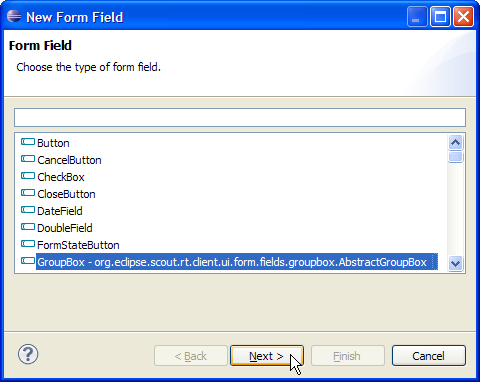
\includegraphics[height=4.5cm]{sdk_new_field_groupbox_1.png} \hspace{8mm}
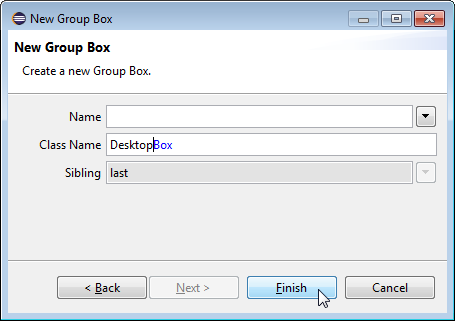
\includegraphics[height=4.5cm]{sdk_new_field_groupbox_2.png}
\caption{Adding the \textit{DesktopBox} field with the Scout SDK form field wizard.}
\index{SDK Wizard!New Form Field}
\figlabel{helloworld_groupboxfield}
\end{figure}

We can now add the text field widget to the group box just created.
To do this, we expand the \element{MainBox} in the Scout Explorer view to access the newly created \element{DesktopBox} element. 
On the \element{DesktopBox} we can then use the \menu{New Form Field ...} again.
In the first wizard step, we select \element{StringField} as the form field type. 
To select the \element{StringField} type you can either scroll down the list of available types or enter ''st'' into the field above the field type list. 

In the second wizard step, we enter 'Message' into the \field{Label}.
As we do not yet have the text 'Message' available in our ''Hello World'' application the wizard prompts the user with the proposal \textsc{New Translated Text ...}.
With a double click on this option a new text entry can be added to the application as shown in \figref{helloworld_stringfield}.
Once we have provided some initial translation for our message label, we can close the translation dialog with the \button{Ok}.
Finally, we close the form field wizard using the \button{Finish}.

\begin{figure}
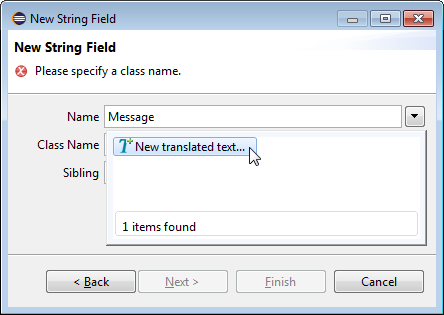
\includegraphics[height=4.2cm]{sdk_new_field_stringfield_1.png} \hspace{8mm}
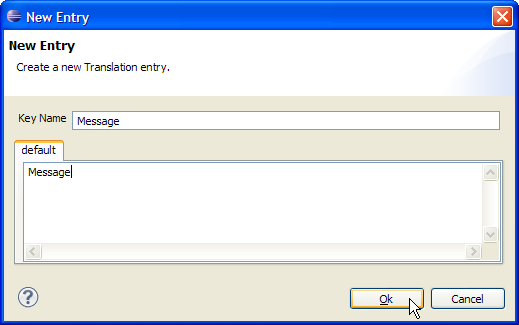
\includegraphics[height=4.2cm]{sdk_new_field_stringfield_2.png}
\caption{Adding a \textit{StringField} and providing a new translation entry.}
\index{SDK Wizard!Add Translation Entry}
\figlabel{helloworld_stringfield}
\end{figure}

By expanding the \element{DesktopBox} element in the Scout Explorer, the new message field becomes visible. 
A double click on the message field element then loads the corresponding Java code into an Editor and displays the message field's properties in the Scout Object Properties as shown in \figref{helloworld_messagefield}.
This is a good moment to compare your status with this screenshot.
Make sure that both the Java code and the project structure in the Scout Explorer look as shown in \figref{helloworld_messagefield}. 

\begin{figure}
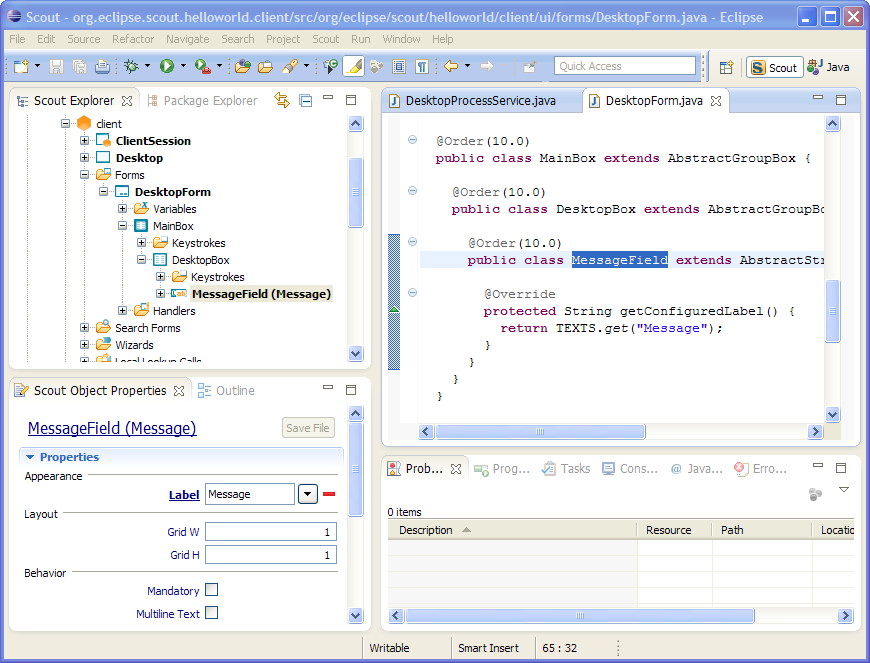
\includegraphics[width=15cm]{sdk_helloworld_messagefield.png}
\caption{Scout SDK showing the \it{MessageField}}
\figlabel{helloworld_messagefield}
\end{figure}

Having verified your status of the ''Hello World'' application you can start the application as described in the previous section.
The client applications will then display your message widget.
However, the text widget is still empty, as we did not yet load any initial content into it.
This is the topic of the next section where we continue this tutorial with the server part.

% =========================================================================== %
% EOF TeX input file
% =========================================================================== %


% --------------------------------------------------------------------------- %
\section{The Server Part}
\seclabel{helloworld.server}

% =========================================================================== %
% TeX input file: "Create the hello world backend"
%
% WARNING: this tex file does not compile standalone, it needs to be embedded
% in a master tex document (e.g. Introduction.tex)
% =========================================================================== %

The responsibility of the Scout server in our ''Hello World'' application is to provide an initial text content for the message field in the client's user interface.
We implement this behaviour in the \java{load} method of the server's \java{DesktopService}.
An empty stub for the \java{load} method of the \java{DesktopService} service has already been created during the initial project creation step. 

To navigate to the implementation of the desktop service in the Scout SDK, we first expand the blue top-level \node{server} in the Scout Explorer.
Below the server node, we then expand the \folder{Services} which shows the \element{DesktopService} element.
Expanding this \element{DesktopService} node, the \java{load} method becomes visible as shown in \figref{helloworld_load_servicemethod}.

\begin{figure}
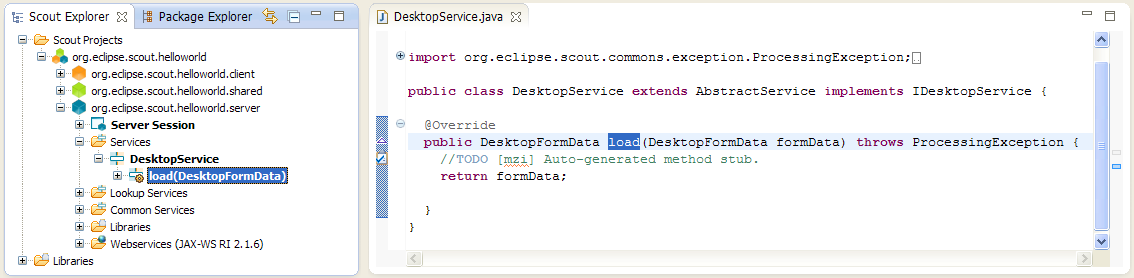
\includegraphics[width=14cm]{sdk_server_desktopservice_load.png}
\caption{The Scout Explorer showing the blue server node expanded with the \folder{Services}.
In this folder the \element{load} method of \element{DesktopService} is selected and its initial implementation is shown in the editor on the right side.}
\figlabel{helloworld_load_servicemethod}
\end{figure}

The \java{DesktopService} represents the server service corresponding to the \java{DesktopForm} on the client side.
This initial setup represents Scout's default where client forms and server services typically come in pairs.
Whenever the client's user interface displays a form to the user, the client connects to the server and calls the \java{load} method of the corresponding server service.
We just need to add our business logic to the \java{load} method of the server's \java{DesktopService}.

According to the signature of the \java{load} method, a \java{formData} object is passed into this method that is then handed back in the return statement.
To complete the implementation of the \java{load} method it is sufficient to assign the text 'hello world!' to the message field part of the form data according to the following line.

\begin{lstlisting}[backgroundcolor=\color{white}]
// test comment
formData.getMessage().setValue("Hello World!");
\end{lstlisting}

The complete implementation of the load method is provided below.
With this last element we have completed the Scout ''Hello World'' application.

\begin{lstlisting}
@Override
public DesktopFormData load(DesktopFormData formData) 
    throws ProcessingException 
{
    formData.getMessage().setValue("Hello World!"); 
    return formData;
}
\end{lstlisting}

% =========================================================================== %
% EOF TeX input file
% =========================================================================== %


% --------------------------------------------------------------------------- %
\section{Add the Rayo Look and Feel}

\begin{figure}
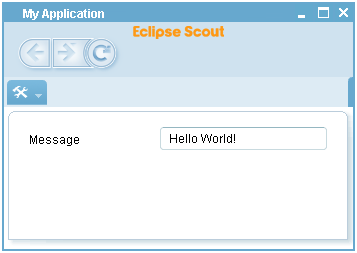
\includegraphics[width=7cm]{helloworld_message_swing_rayo.png} \hspace{5mm}
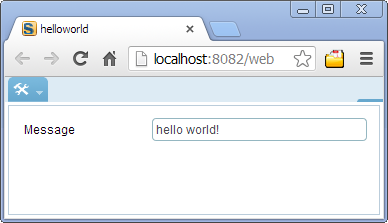
\includegraphics[width=7cm]{helloworld_message_rap_rayo.png}
\caption{The ''Hello World'' client application with the Rayo look and feel. The desktop client is shown on the left and the web client on the right hand side.}
\figlabel{helloworld_clientapp}
\end{figure}

For Eclipse Scout applications a slick look and feel called Rayo is available in the Eclipse Marketplace\footnote{
Eclipse Marketplace: \url{http://marketplace.eclipse.org/}
}.
And in this (optional) part of the ''Hello World'' tutorial we will add Rayo to our ''Hello World'' Swing client application.
As a result, we will get a Scout desktop application that looks the same as the corresponding Scout web client as shown in \figref{helloworld_clientapp}.

\begin{figure}
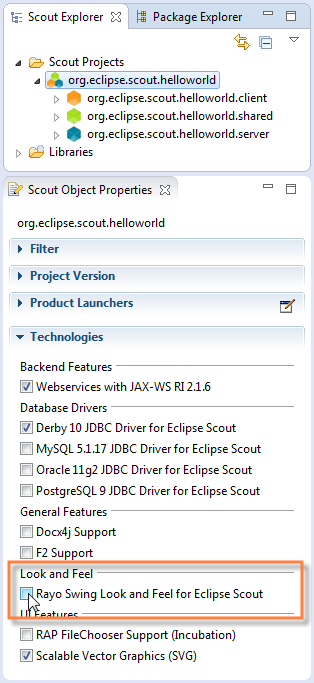
\includegraphics[width=6cm]{sdk_rayo_add_checkbox.png} \hspace{5mm}
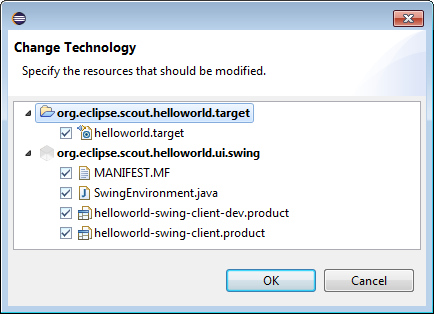
\includegraphics[width=8cm]{sdk_rayo_confirm_changes.png}
\caption{Adding the Rayo Swing look and feel. The Rayo checkbox to activate the look and feel is highlighted on the left hand side. The dialog on the right hand side shows the changes in the Swing plugin and the target file that will be made by the Scout SDK.}
\figlabel{selecting_rayo}
\end{figure}

To add Rayo in the Scout SDK to our ''Hello World'' project, switch to the Scout Explorer and select the top-level \node{org.eclipse.scout.helloworld}.
Then, according to \figref{selecting_rayo}, select the checkbox \element{Rayo Swing Look and Feel for Eclipse Scout} under the \element{Technologies} section of the Scout Object Properties.
This brings up a dialog showing the proposed changes to application's target file and the Swing plugin of the ''Hello World'' application. 
These changes need to be confirmed with the \button{OK}.
The first time the user adds the Rayo feature in the Scout SDK, Eclipse needs to download the package from the Eclipse Marketplace.
This download and subsequent installation of Rayo will make you to go through the following steps.

\begin{enumerate}
  \item Accept Licence: GPL with Classpath Exception
  \item Accept unsigned content
\end{enumerate}

After the successful download and installation of the Rayo package, start the Swing client using the procedure described in \secref{run_initial}.
When we also start the web client of the ''Hello World'' application using the RAP product launcher, we can compare the result side by side.

% --------------------------------------------------------------------------- %
\section{Exporting the Application}
\seclabel{helloworld_export}

We are now ready to move the finished ''Hello World'' application from our development environment to a productive setup.
The simplest option to move our application into the 'wild' is to use the \wizard{Export Scout Project} provided by the Scout SDK.
Using the default settings, the export wizard produces two WAR files\footnote{
Web application ARchive (WAR): \url{http://en.wikipedia.org/wiki/WAR_file_format_(Sun)}
}
that contain the complete Scout server and the desktop and mobile client applications.

To deploy the application to a web server the WAR files generated by the wizard are the only artefacts needed.
The first WAR file contains the Scout server including a zipped desktop client for downloading.
In the second WAR file, the RAP server application that provides both the web client and the client for mobile devices.

\begin{figure}
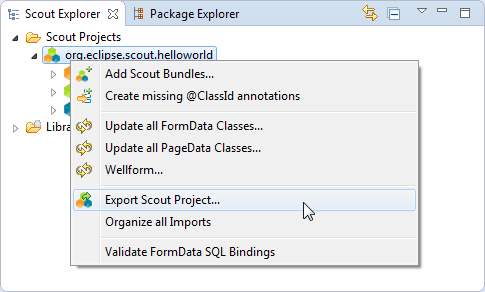
\includegraphics[width=8cm]{sdk_export_war_menu.png} 
\caption{Starting the \wizard{Export Scout Project} in the Scout SDK with the context menu. 
In the first wizard step, the target directory for the WAR files and the artefacts to export are specified.}
\index{SDK Wizard!Export Scout Project}
\figlabel{sdk_export_war}
\end{figure}

\begin{figure}
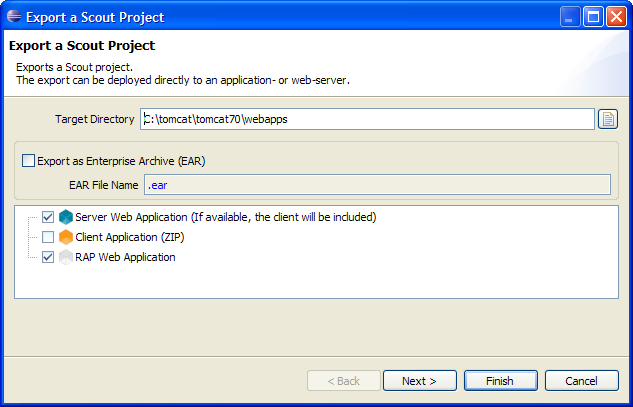
\includegraphics[width=12cm]{export_wizard_1.png}
\caption{The first dialog of the \wizard{Export Scout Project}. 
Here, the target directory for the WAR files that will be generated by the wizard is specified.}
\figlabel{export_wizard_1}
\end{figure}

To start the export wizard, we start the Scout SDK with the ''Hello World'' Scout project.
In the Scout Explorer we then select the corresponding \contextmenu{Export Scout Project...} on the ''Hello World'' top level application node as shown in \figref{sdk_export_war}.
In the first wizard dialog shown in \figref{export_wizard_1}, the target directory for the WAR files needs to be specified.
You may choose any directory as the target directory\footnote{
Make sure to remember the location of this directory.
We will need the directory location again when we deploy these WAR files to the Tomcat web server.
}.
After clicking \button{Next} the second wizard step proposes the server product file that specifies the artefacts to be exported including the file name for the WAR file for the ''Hello World'' server application.
Typically, the proposed default values are fine.
Move to the third dialog with \button{Next}.

\begin{figure}
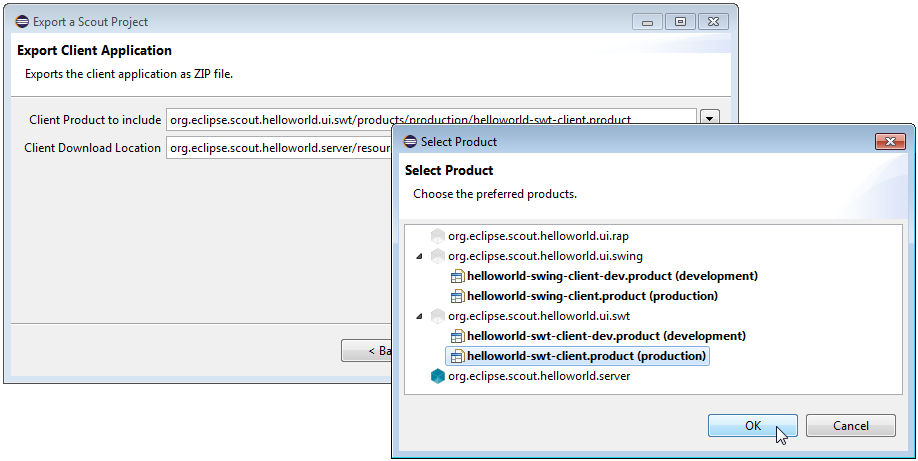
\includegraphics[width=13cm]{export_wizard_3.png}
\caption{The third dialog of the \wizard{Export Scout Project} defines the client application to be included in the \texttt{helloworld\_server.war} file.
In the last step of the export wizard the RAP sever is exported to the specified file name (right).}
\figlabel{export_wizard_3}
\end{figure}

In the third dialog of the \wizard{Export Scout Project} the desktop client to be included in the WAR file needs to be specified.
The default selection is set to the SWT client application.
For the ''Hello World'' example, we want to include the Swing client application with the Rayo Look and Feel.
For this, we need to change the selected product to \element{helloworld-swing-client.product (production)} according to \figref{export_wizard_3}.
With \button{Next} we move to the last wizard step.

\begin{figure}
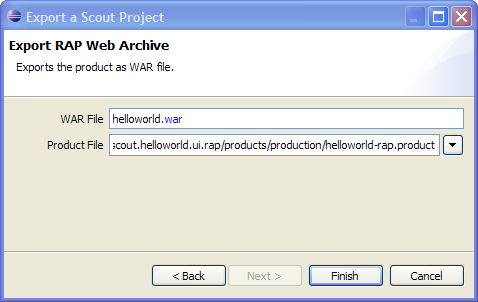
\includegraphics[width=12cm]{export_wizard_4.png}
\caption{The last dialog of the \wizard{Export Scout Project} defines the export of the RAP server.
Normally, the proposed field values do not need any adjustments.}
\figlabel{export_wizard_4}
\end{figure}

In the last wizard dialog shown in \figref{export_wizard_4}, the RAP server product and the corresponding WAR file name are specified.
Normally, the proposed field values are fine and we can close the wizard with \button{Finish}.
After this last step, the Scout SDK is assembling the necessary artefacts and building the two ''Hello World'' WAR files.
These two WAR files are the only items needed for deploying the ''Hello World'' application to a web server

% --------------------------------------------------------------------------- %
\section{Deploying to Tomcat}
\seclabel{helloworld_deploy}

As the final step of this tutorial, we deploy the two WAR files representing our ''Hello World'' application to a Tomcat web server.
For this, we first need a working Tomcat installation.
If you do not yet have such an installation you may want to read and follow the instructions provided in \appref{install_tomcat}.
To verify a running Tomcat instance, type \url{http://localhost:8080/} into the address bar of the web browser of your choice.
You should then see the page shown in \figref{deploy_tomcat_1}.

\begin{figure}
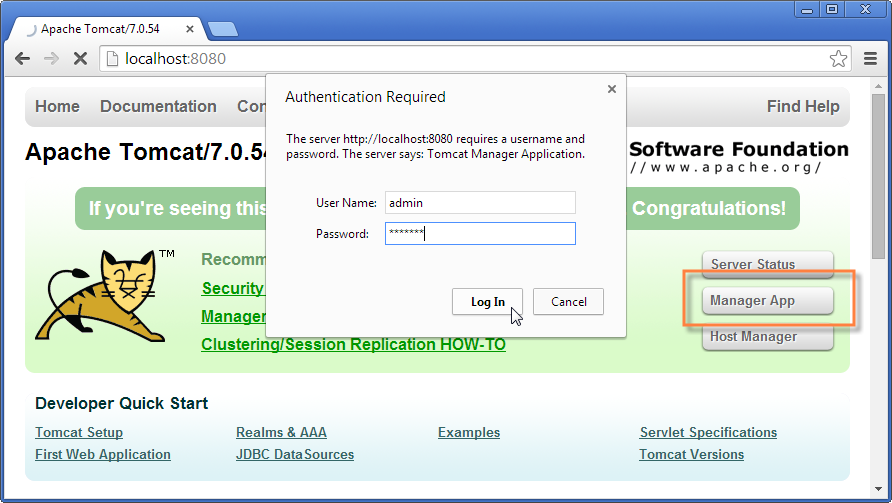
\includegraphics[width=15cm]{tomcat_managerapp_login.png} 
\caption{The Tomcat shown after a successful installation. 
After clicking on the ''Manager App'' button (highlighted in red) the login box is shown in front.
A successful login shows the ''Tomcat Web Application Manager''.}
\figlabel{deploy_tomcat_1}
\end{figure}

\begin{figure}
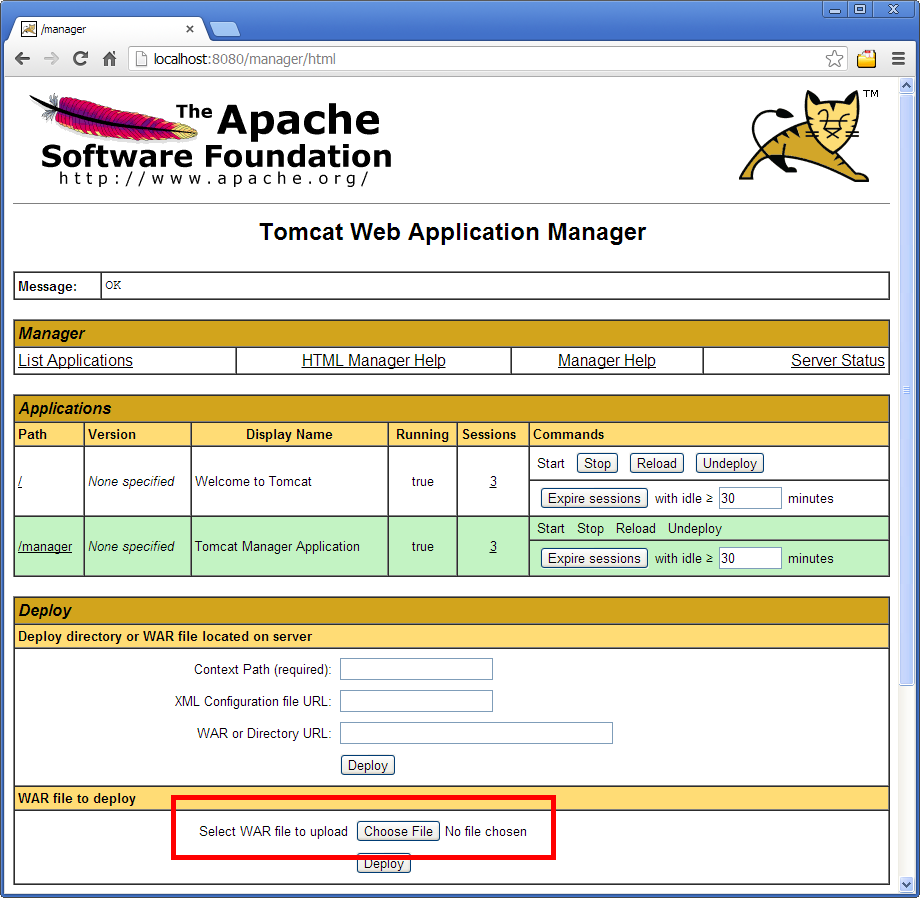
\includegraphics[width=15cm]{tomcat_managerapp_selectwar.png}
\caption{The ''Tomcat Web Application Manager''.
The WAR files to be deployed can then be selected using button ''Choose File'' highlighted in red.}
\figlabel{deploy_tomcat_2}
\end{figure}

Once the web browser displays the successful running of your Tomcat instance, switch to its ''Manager App'' by clicking on the button highlighted in \figref{deploy_tomcat_1}.
After entering user name and password the browser will display the ''Tomcat Web Application Manager'' as shown in \figref{deploy_tomcat_2}.
If you don't know the correct username or password you may look it up in the file \filename{tomcat-users.xml} as described in \appref{tomcat_dirs_and_files}.

After logging successfully into Tomcat's manager application, you can select the WAR file(s) to be deployed using button ''Choose File'' according to the right hand side of \figref{deploy_tomcat_2}.
After picking your \filename{helloworld_server.war} and \filename{helloworld.war} file and closing the file chooser, click on button ''Deploy'' (located below button ''Choose File'') to deploy the application to the Tomcat web server.
This will copy the selected WAR file into Tomcats \filename{webapps} directory and unpack its content into a subdirectory with the same name.
Deploying the file \filename{helloworld.war} will extract its contents into a subdirectory named \filename{helloworld}.
And the file \filename{helloworld_server.war} will be extracted into subdirectory \filename{helloworld_server}.
You can now connect to the deployed application using the browser of your choice and enter the following address.

\begin{lstlisting}
  http://localhost:8080/helloworld_server/
\end{lstlisting}

\begin{figure}
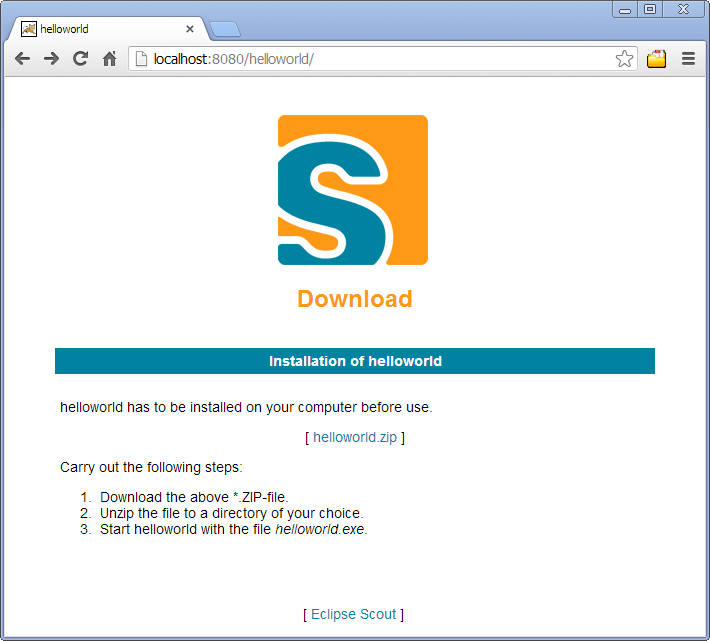
\includegraphics[width=15cm]{tomcat_helloworld_download.png}
\caption{The ''Hello World'' home page, providing a link to download the desktop client.}
\figlabel{helloworld_running_download}
\end{figure}

You will then see the home page of the server of your ''Hello World'' application shown in \figref{helloworld_running_download}.
From here you can download the zipped client application that can be saved in a directory of your choice.
After unpacking the zip file, you may start the executable file named \filename{helloworld}.
This will start the ''Hello World'' client application as shown on the left hand side of \figref{helloworld_running_clients}.
To start the ''Hello World'' web application, open a browser and enter the following address.

\begin{lstlisting}
  http://localhost:8080/helloworld/
\end{lstlisting}

\begin{figure}
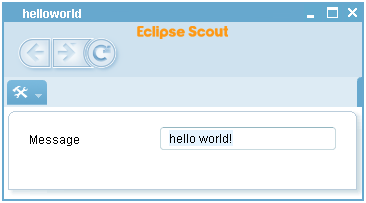
\includegraphics[height=2.5cm]{helloworld_finished_rayo_swing.png}\hspace{5mm}
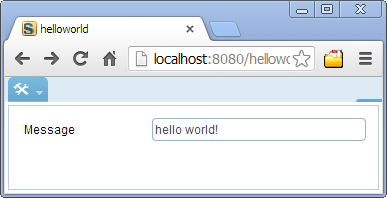
\includegraphics[height=2.5cm]{helloworld_finished_rayo_rap.png}\hspace{5mm}
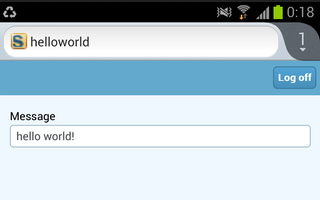
\includegraphics[height=2.5cm]{helloworld_finished_rayo_rap_mobile.png}
\caption{The ''Hello World'' client application running on the desktop, in the browser and on a mobile device.}
\figlabel{helloworld_running_clients}
\end{figure}

Depending on the device your browser is running on you will be redirected to \texttt{helloworld/web} on a desktop or laptop computer, to \texttt{helloworld/mobile} on a mobile device or to \texttt{helloworld/mobile} if you are connecting from a tablet device.
\figref{helloworld_running_clients} shows screenshots for a desktop client, the web application and the same application in a mobile browser.
As demonstrated in these screenshots \texttt{helloworld/web} and \texttt{helloworld/mobile} lead to a different presentation of the same UI optimized to the target form factors of desktop browsers, tablets, and mobile phones.

% =========================================================================== %
\chapter{''Hello World'' Background}
\chalabel{helloworld_background}

The previous ''Hello World'' tutorial has been designed to cover the creation of a complete client server application in a minimal amount of time.
In this chapter, we will take a deeper look at the ''Hello World'' and provide background information along the way.
The goal is to explain many of the used concepts in the context of a concrete Scout application to allow for a well rounded first impression of the Eclipse Scout framework and the tooling provided by the Scout SDK.

The structure of this chapter is closely related to the ''Hello World'' tutorial.
As you will notice, the order of the material presented here exactly follows the previous tutorial and identical section titles are used where applicable.
In addition to \charef{helloworld}, we include \secref{initial_helloworld} to discuss the initial application generated by the Scout SDK.

% --------------------------------------------------------------------------- %
\section{Create a new Project}
\seclabel{create_project_simple_background}

The first thing you need for the creation of a new Scout project is to select a new workspace.
For Eclipse, a workspace is a directory where Eclipse can store a set of projects in a single place.
As Scout projects typically consist of several Eclipse plugin projects the default (and recommended) setting is to use a single workspace for a single Scout project.

\begin{figure}
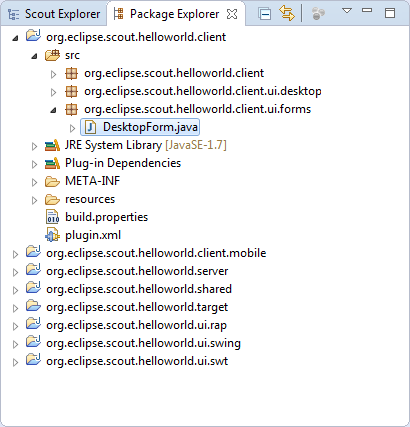
\includegraphics[width=7cm]{sdk_package_explorer.png} \hspace{0.5cm}
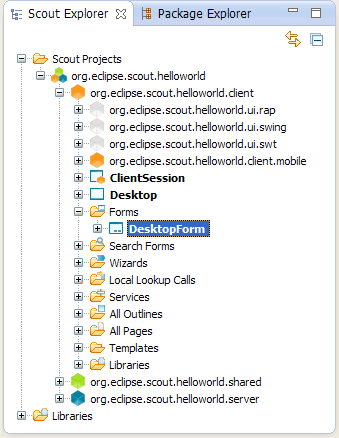
\includegraphics[width=7cm]{sdk_scout_explorer.png}
\caption{The Eclipse plugin projects of the ''Hello World'' application shown by the Package Explorer in the Scout SDK on the left hand side. 
The corresponding view in the Scout Explorer is provided on the right hand side.
}
\figlabel{package_explorer}
\end{figure}

In the case of the ''Hello World'' application, the workspace contains seven plugin projects as shown on the left side of \figref{package_explorer}.
In the expanded source folder of the client plugin \element{org.eclipse.scout.helloworld.client} the organisation of the Java packages is revealed.
The Scout Explorer provided on the right side of \figref{package_explorer} shows three colored top level nodes below the main project \element{org.eclipse.scout.helloworld}.

In the Scout Explorer, the main project node expands to the orange client node \element{org.eclipse.scout.helloworld.client}, the green shared node \element{org.eclipse.scout.helloworld.client} and the blue server node \element{org.eclipse.scout.helloworld.server}.
The client node first presents the white user interface (UI) nodes \element{org.eclipse.scout.helloworld.client.ui.*} indicating the supported UI technologies.
Next, the client mobile node \element{org.eclipse.scout.helloworld.client.mobile} is shown.
It is responsible for adapting the layout of the user interface suitably for mobile and tablet devices.
Finally, after the \node{ClientSession} and the \node{Desktop}, component specific folders allow for a simple navigation to the various client parts.

Comparing the Package Explorer with the Scout Explorer a couple of aspects are notable.
First, the number and names of the Eclipse plugin projects is identical in both the Package Explorer and the Scout Explorer view.
However, the Scout Explorer recognizes the Scout project structure and explicitly renders the relation between the different Eclipse plugins.
In addition, individual node colors are used to indicate the role of each plugin project.
Second, the focus of the Scout Explorer lies on the business functionality of the complete client server application.
Artefacts only necessary to the underlying Eclipse platform are not even accessible.
Third, on the individual elements rendered in the Scout Explorer, the Scout SDK provides menus to start wizards useful to the selected context.
In the case of the ''Hello World'' tutorial we could create the complete application (except for a single line of Java code) using these wizards .

When we revisit the \wizard{New Scout Project} in \figref{sdk_new_project_wizard}, it now becomes trivial to explain how the \field{Project Name} \java{org.eclipse.scout.helloworld} was used as the common prefix for plugin project names and Java package names.
Based on the project name, the last part \java{helloworld} was used for the \field{Project Alias}.
As we have seen in \secref{helloworld_export}, this project alias is used by the Scout SDK to build the base names of the WAR files in the export step.
In turn, after deploying the WAR files as described in \secref{helloworld_deploy}, the RAP server application becomes available under the URL \java{http://localhost:8080/helloworld}.
Should you have a catchy naming for you application in mind, \java{com.mycompany.mycatchyname} is therefore a good choice for the \field{Project Name}.


% --------------------------------------------------------------------------- %
\section{Walking through the Initial Application}
\seclabel{initial_helloworld}

In this section, we will walk you through the central Scout application model components of the ''Hello World'' example. 
As each of these components is represented by a Java class in the Scout framework, we can explain the basic concept using the available ''Hello World'' source code.
Below, we will introduce the following Scout components.

\begin{itemize}
  \item Desktop
  \item Form
  \item Form handler
  \item Service
  \item MainBox
  \item Form data
  \item Form field
\end{itemize}

Please note that most of the Java code was initially generated by Scout SDK.
In many cases this code can be used ''as is'' and does not need to be changed.
Depending on your requirements, it might very well be that you want to adapt the provided code to fit your specific needs.
However, a basic understanding of the most important Scout components should help you to better understand the structure and working of Scout applications.

% ........................................................................... %
\subsection{Desktop}

The desktop is the central container of all visible elements of the Scout client application.
It inherits from Scout class \java{AbstractDesktop} and represents the empty application frame with attached elements, such as the applications menu tree.
In the ''Hello World'' application, it is the Desktop that is first opened when the user starts the client application.

To find the desktop class in the Scout Explorer, we first navigate to the orange \node{client} and double click the \node{Desktop} just below.
This will open the associated Java file \texttt{Desktop.java} in the editor view of the Scout SDK.
Of interest is the overwritten callback method \java{execOpened} shown in \lstref{helloworld.execopened}.

\lstinputlisting[
  label=\lstlabel{helloworld.execopened},
  caption=Creating and starting a form in the client's Desktop callback method \java{execOpened}.,
  index={DesktopForm},
  linerange={32-41},
  float
]
{../code/helloworld/org.eclipse.scout.helloworld.client/src/org/eclipse/scout/helloworld/client/ui/desktop/Desktop.java}

Method \java{execOpened} is called by the Scout framework after the desktop frame becomes visible.
The only thing that happens here is the creation of a \java{desktopForm} object, that gets assigned an icon before it is started via method \java{startView}.
This desktop form object holds the \field{Message} text widget that is displayed to the user\footnote{
In the Scout application model we can only add UI fields to Scout form elements, not directly to the desktop.
}.
More information regarding form elements are provided in the next section.

% ........................................................................... %
\subsection{Form}
\seclabel{helloworld.form}

Scout forms are UI containers that hold form field widgets.
A Scout form always inherits from Scout class \java{AbstractForm} and can either be displayed as a dialog in its own window or shown as a view inside of another UI container.
In the ''Hello World'' application a \java{DesktopForm} object is created and displayed as a view inside of the desktop element.

To find the desktop form class in the Scout Explorer, expand the orange \node{client}\footnote{
To expand elements (nodes, folders, etc.) in the Scout Explorer, use a double click on the element or a single click on the plus icon in front of the element.}.
Below this node, you will find the \folder{Forms}. 
Expand this folder to show the \element{DesktopForm} as shown in \figref{helloworld_viewhandler}.
In the Scout Object Property window in the screenshot, we can also see the \property{Display Hint}.
Its value is set to 'View' to display the desktop form as a view and not as a dialog in its own frame.

\begin{figure}
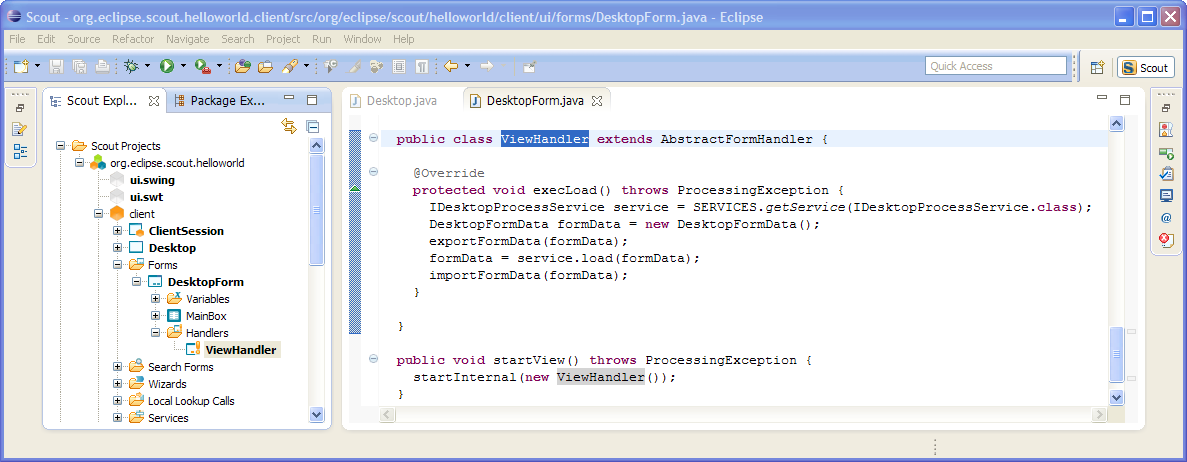
\includegraphics[width=15cm]{sdk_helloworld_viewhandler.png}
\caption{Scout SDK showing the DesktopForm's \textit{ViewHandler} in the Scout Explorer and the properties of the DesktopForm in the Scout Object Properties.}
\figlabel{helloworld_viewhandler}
\end{figure}

Expand the \element{DesktopForm} to show its children: \element{Variables}, \element{MainBox} and \element{Handlers}.
The \element{Variables} sub folder contains variables. They are invisible to the application user.
The ''Hello World'' application is so simple, it does not need variables.
The sub folder \element{MainBox} contains form fields. These are the visible user interface elements.
The main box of our \java{DesktopForm} holds the \java{DesktopBox} containing the \java{MessageField} added with the \wizard{New Form Field}.
Finally, the \element{Handlers} sub folder contains all available form handlers.
The view handler shown in \figref{helloworld_viewhandler} has been added in the initial project creation step.

% ........................................................................... %
\subsection{Form Handler}
\seclabel{helloworld.formhandler}

Form handlers are used to manage the form's life cycle.
Scout form handlers inherit from \java{AbstractFormHandler} and allow the implementation of desired behaviour before a form is opened, or after it is closed.
This is achieved by overwriting callback methods defined in \java{AbstractFormHandler}.
The necessary wiring is provided by the Scout framework, either by the initial project creation step or when using one of the provided Scout SDK wizards.

\lstinputlisting[
  label=\lstlabel{helloworld.viewhandler},
  caption=Class \java{DesktopForm} with its view handler and \java{startView} method. Other inner classes and methods are omitted here.,
  index={ViewHandler},
  emph={load},
  linerange={19-20,86-103},
  float
]
{../code/helloworld/org.eclipse.scout.helloworld.client/src/org/eclipse/scout/helloworld/client/ui/forms/DesktopForm.java}

In the ''Hello World'' application, it is the overwritten \java{execLoad} method in the \java{ViewHandler} that defines what will happen before the desktop form is shown to the user.
The corresponding source code is provided in \lstref{helloworld.viewhandler}.
It is this \java{execLoad} method where most of the behaviour relevant to the ''Hello World'' application is implemented.
Roughly, this implementation is performing the following steps.

\begin{enumerate}
  \item Get a reference to the forms server service running on the server.
  \item Create a data transfer object (DTO)\footnote{
Data Transfer Object (DTO): \url{http://en.wikipedia.org/wiki/Data_transfer_object}.}
  \item Pass the empty DTO to the load service method (ask the server for some data).
  \item Update the DTO with the content provided by the service load method.
  \item Copy the updated information from the DTO into the desired form field.
\end{enumerate}

To open the \java{ViewHandler} class in the Java editor of the Scout SDK, double click on the \element{ViewHandler} in the Scout Explorer.
Your Scout SDK should then be in a state similar to \figref{helloworld_viewhandler}.
In the lower part of \lstref{helloworld.viewhandler} we can see the wiring between the desktop form and the view handler in method \java{startView}.
Further up, we find method \java{execLoad} of the view handler class.

Before we discuss this method's implementation, let us examine when and how \java{execLoad} is actually called.
As we have seen in the \java{Desktop} class (see \lstref{helloworld.execopened}), the form's method \java{startView} is executed after the desktop form is created.
Inside method \java{startView} (see \lstref{helloworld.viewhandler}), the desktop form is started/opened using \java{startInternal}.
In method \java{startInternal} a view handler is then created and passed as a parameter.
This eventually leads to the call of our \java{execLoad} custom implementation.

We are now ready to dive into the implementation of method \java{execLoad} of the desktop form's view handler.
First, a reference to a form service identified by \java{IDesktopService} is obtained using \java{SERVICES.getService}.
Then, a form data object (the DTO) is created and all current form field values are exported into the form data via method \java{exportFormData}.
Strictly speaking, the \java{exportFormData} is not necessary for the use case of the ''Hello World'' application.
But, as this is generated code, there is no benefit when we manually delete the \java{exportFormData} command.
Next, using the \java{load} service method highlighted in \lstref{helloworld.viewhandler}, new form field values are obtained from the server and assigned to the form data object.
Finally, these new values are imported from the form data into the form via the \java{importFormData} method.
Once the desktop form is ready, showing it to the user is handled by the framework.

To add some background to the implementation of the \java{execLoad} above, the next section introduces services and form data objects. 

% ........................................................................... %
\subsection{Form Services and Form Data Objects}

Form services and form data objects are used in the Scout framework to exchange information between the Scout client and server applications.
When needed, a service implemented on the server side can register a corresponding proxy service on the client.
This proxy service is invoked by the client as if it were implemented locally.
In fact, when we get a service reference using \java{SERVICES.getService}, we do not need to know if this service runs locally on the client or remotely on the server.

In the ''Hello World'' example application, the client's desktop form has an associated desktop service running on the server.
This correspondence between forms and form services is also reflected in the \element{Links} section of the Scout Object Properties of the desktop form.
As shown in \figref{helloworld_viewhandler}, links are provided not only for the desktop form, but for its desktop form data, the corresponding desktop form service as well as for the service interface \java{IDesktopService}. 
On the client, this interface is used to identify and register the proxy service for the desktop service.

To transfer data between the client and the server, the ''Hello World'' application uses a \java{DesktopFormData} object as a DTO.
This form data object holds all form variables and values for all the form fields contained in the form.
Taking advantage of this correspondence, the Scout framework provides the convenience methods \java{exportFormData} and \java{importFormData}.
As a result, the developer does not need to deal with any mapping code between the form data object and the form fields.

The actual implementation of the desktop form service in class \java{DesktopService} is implemented on the server side.
As the class \java{DesktopService} represents an ordinary Scout service it inherits from \java{AbstractService}.
It also implements its corresponding \java{IDesktopService} interface used for registering both the actual service as well as the proxy service.

% --------------------------------------------------------------------------- %
\section{Run the Initial Application}
\seclabel{run_initial_background}

% ........................................................................... %
\subsection{The Launcher Boxes}

To run a Scout application the Scout SDK provides launcher boxes in the Scout Object Properties as described in \secref{run_initial}.
These object properties are associated to the top level project node in the Scout Explorer.
Using the \icon{Edit} provided in the product launcher section of the Scout Object Properties, the list of launcher boxes can be specified as shown in \figref{select_product_launchers}.

\begin{figure}
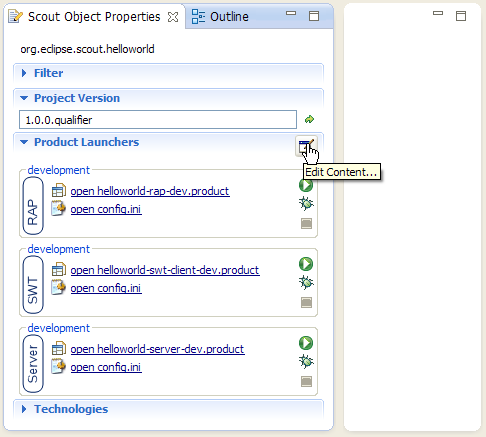
\includegraphics[height=6.5cm]{sdk_edit_product_launcher.png} \hspace{0.5cm}
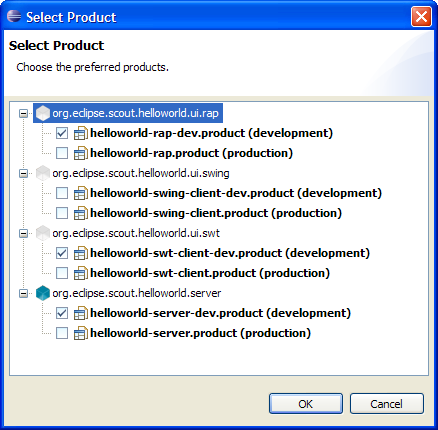
\includegraphics[height=6.5cm]{sdk_select_product_launcher.png}
\caption{Using the \icon{Edit Content...} shown on the left hand side, the product selection dialog shown on the right side is opened.
Using this product selection dialog, the list of launcher boxes can be specified.
}
\figlabel{select_product_launchers}
\end{figure}

% ........................................................................... %
\subsection{Eclipse Product Files}

The available products shown on the right side of \figref{select_product_launchers} represent the Eclipse product files created in the initial project creation step.
Product files\footnote{
Read the following article for an introduction to Eclipse product files: \url{http://www.vogella.com/articles/EclipseProductDeployment/article.html}.
}
are used in Eclipse to specify the configuration and content of an executable application.
In the case of the ''Hello World'' project, four executable applications --- with two Eclipse product files for each application --- have been defined by the Scout SDK.
The four applications, one for the server application and one for each client technology, have already been discussed in \secref{run_initial}.

\begin{figure}
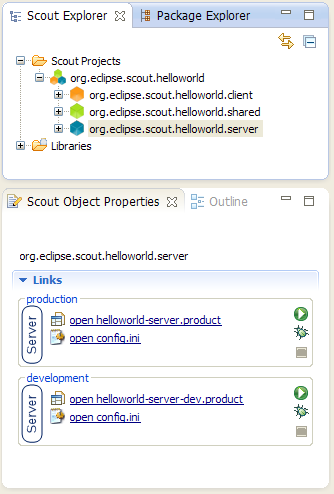
\includegraphics[height=8.5cm]{sdk_server_node_properties.png} \hspace{0.5cm}
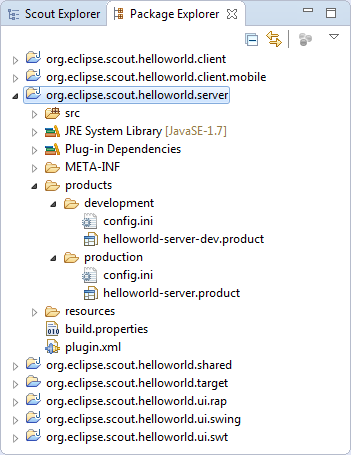
\includegraphics[height=8.5cm]{sdk_server_plugin_explorer.png}
\caption{The production and development launcher boxes associated with the ''Hello World'' server application are shown on the left side. 
In the Package Explorer shown on the right side, the production and development products are located under the \folder{products} in the server plugin project.
}
\figlabel{server_plugin}
\end{figure}

We assume that Scout applications will be run in at least two different environments.
Once from within the Eclipse IDE in the development environment, and once by the actual end users outside the Eclipse IDE. 
This second environment is named production environment. 
Depending on the complexity of deployment processes there might be some more environments to consider, such as testing and integration environments. 
This is the reason that the Scout SDK initially creates two product files that are associated with the development and the production environment.

Even in the case of the simple ''Hello World'' example, the Scout application is started in two target environments.
The development environment defines the product in the context of the Scout SDK.
To export and run the Scout application outside of the Scout SDK, the production product files are used to define the application when it is to be started on a Tomcat web server.
\figref{server_plugin} illustrates this situation for the ''Hello World'' server application. 
On the left side, the blue server node is selected in the Scout Explorer.
This opens the two server launcher boxes for the production and the development environment.
On the right side of \figref{server_plugin}, the corresponding plugin project \element{org.eclipse.scout.helloworld.server} is expanded to show the file based organisation of the two product definitions.

\begin{figure}
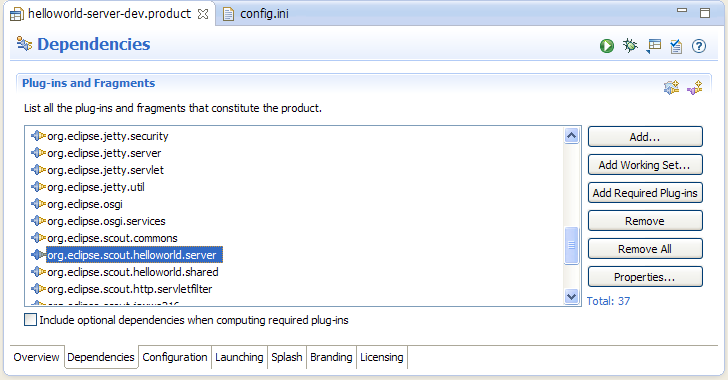
\includegraphics[width=14cm]{sdk_server_dev_product.png} 
\caption{The Eclipse product file editor showing file \java{helloworld-server-dev.product} of the ''Hello World'' application.
In the Dependencies tab shown above, the list of Eclipse plugins that are required for the server application are shown.
}
\index{Eclipse product file editor}
\figlabel{server_dev_product}
\end{figure}

For the case of the ''Hello World'' example we did not need to edit or change the product files generated by the Scout SDK. 
However, if your requirements are not met by the provided product files, you may use the Eclipse product file editor.
A screenshot of this editor is shown in \figref{server_dev_product} with the tab \element{Dependencies} opened.
In the tab Dependencies, the complete list of necessary plugins is provided.
Example plugins visible in \figref{server_dev_product} include the ''Hello World'' server and shared plugins, Scout framework plugins, and Jetty plugins.
The Jetty\footnote{
Jetty is web server with a small footprint: \url{http://www.eclipse.org/jetty/}.
} 
plugins are only needed to run the ''Hello World'' server application inside the Scout SDK.
Consequently, Jetty plugins are not listed as a dependency in the Scout server's production product file.

% ........................................................................... %
\subsection{Eclipse Configuration Files}
\index{Eclipse \filename{config.ini} file}
\seclabel{config_ini}

\begin{figure}
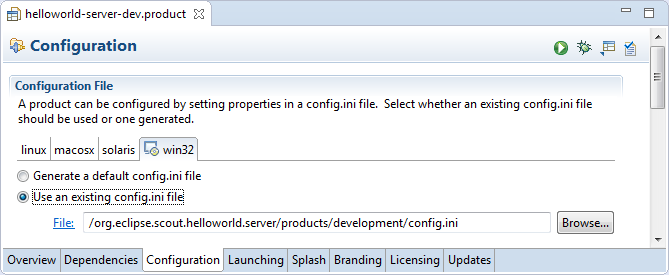
\includegraphics[width=14cm]{sdk_server_dev_product_config.png} \\ 

\includegraphics[height=5mm]{white_pixel.png} \\
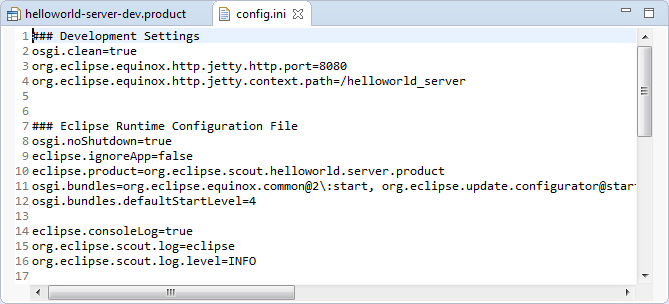
\includegraphics[width=14cm]{sdk_server_dev_configini.png} 
\caption{Above, the definition of the products \java{config.ini} in tab \element{Configuration} of the product file editor.
Below, the content of the configuration file of the ''Hello World'' server application is provided in a normal text editor.
}
\figlabel{server_dev_ini}
\end{figure}

Switching to tab \element{Configuration} in the product file editor, shows the selected radio button \element{Use an existing config.ini file} and the link to the configuration file provided in the \field{File} as shown in the upper part of \figref{server_dev_ini}.
Below, a part of the server's \filename{config.ini} file is shown.
Both the entry in the product file pointing to the configuration file, and the content of the \filename{config.ini} file has been generated by the Scout SDK during the initial project creation step.
As shown in the lower part of \figref{server_dev_ini}, Eclipse configuration files have the format of a standard property file.
The provided key value pairs are read at startup time if the \filename{config.ini} file can be found in folder \filename{configuration} by the Eclipse runtime.

% ........................................................................... %
\subsection{Scout Desktop Client Applications}

Having introduced Eclipse product files and configuration files based on the ''Hello World'' server application, we will now look at the different client applications in turn.
With Swing applications\footnote{
Swing is the primary Java UI technology: \url{http://en.wikipedia.org/wiki/Swing_\%28Java\%29}.
}
and SWT applications\footnote{
Standard Widget Toolkit (SWT): \url{http://en.wikipedia.org/wiki/Standard_Widget_Toolkit}.
}, two alternative UI technologies are currently available to build Scout desktop client applications.
More recently, JavaFX\footnote{
JavaFX is the most recent Java UI technology: \url{http://en.wikipedia.org/wiki/JavaFX}.
} 
is promoted as a successor to Swing and it is therefore likely, that Scout will provide JavaFX client applications in the future.

When we compare the product files for the Swing and the SWT client applications, it is apparent that both client applications share a large number of plugins.
Most importantly, the complete UI model and the business logic is identical for both client applications.
In other words, the value created by the Scout developer is contained in the two plugins \element{org.eclipse.scout.helloworld.client} and \element{org.eclipse.scout.helloworld.shared}.
To create an executable client application, we only need to combine these two plugins with a set of plugins specific to the desired UI technology.

After starting the ''Hello World'' Swing client or the corresponding SWT client application, the client application first reads the startup parameters from its \filename{config.ini} file.
Among other things, this client configuration file contains the parameter \java{server.url} to specify the URL to the ''Hello World'' server. 
After the startup of the ''Hello World'' client application, it can then connect to the ''Hello World'' server application using this address.

% ........................................................................... %
\subsection{Scout Web, Tablet and Mobile Clients}

For Scout web, tablet and  mobile clients, the Eclipse RAP framework\footnote{
Remote Application Platform (RAP): \url{http://www.eclipse.org/rap/}.
}
is used.
\index{RAP}
The RAP framework provides an API that is almost identical to the one provided by SWT and allows to use Java for server-side Ajax\footnote{
Asynchronous JavaScript and XML (AJAX): \url{http://en.wikipedia.org/wiki/Ajax_\%28programming\%29}.
}.
This setup implies that Scout tablet and mobile clients are not native clients but browser based\footnote{
To provide native clients with Scout, the simplest (commercial) option is most likely Tabris: \url{http://developer.eclipsesource.com/tabris/}
}.

Comparing the product file of the SWT client applications with the RAP application, we observe that the RAP development product does not include any SWT plugins, but a set of RAP and Jetty plugins.
In addition, the RAP product also contains the Scout mobile client plugins \element{org.eclipse.scout.rt.client.mobile} and \element{org.eclipse.scout.helloworld.client.mobile}.
These two plugins are responsible for transforming the UI model defined in the ''Hello World'' client plugin to the different form factors of tablet computers and mobile phones.

If you start the ''Hello World'' RAP application in your Scout SDK, you are launching a second server application in a Jetty instance on a different port than the ''Hello World'' server application.
As in the case of the desktop client applications, the RAP or Ajax server application knows how to connect to the ''Hello World'' server application after reading the parameter \java{server.url} from its \filename{config.ini} file.

% --------------------------------------------------------------------------- %
\section{The User Interface Part}
\seclabel{helloworld.userinterface.background}

Using the UI of the ''Hello World'' application we explain in this section how the Scout UI form model is represented in Java. 
We also describe how this representation is exploited by the Scout SDK to automatically manage the form data objects used for data transfer between Scout client and Scout server applications.
Finally, will have a brief look at internationalization\footnote{
Internationalization and localization, also called NLS support: \url{http://en.wikipedia.org/wiki/Internationalization_and_localization}.
} 
support of Scout for texts.

\lstinputlisting[
  label=\lstlabel{helloworld.mainbox},
  caption=The \java{DesktopForm} with its inner class \java{MainBox} containing the desktop box and message field,
  index={MainBox},
  linerange={18-20, 69-85, 102-103},
  float
]
{../code/helloworld/org.eclipse.scout.helloworld.client/src/org/eclipse/scout/helloworld/client/ui/forms/DesktopForm.java}

As discussed in \secref{helloworld.form} Scout forms consist of variables, the main box and a number of form handlers.
The main box represents the visible part of Scout's form model.
It may holds any number of form fields.
Using container fields such as group boxes, it is possible to define complex structures such as hierarchical UI models containing multiple levels.
In the Scout framework the forms structure is represented in the form of inner classes that are located inside of the \java{MainBox} class.
And the \wizard{New Form Field} of the Scout SDK fully supports this pattern.
\lstref{helloworld.mainbox} provides the concrete example using the the desktop form of the ''Hello World'' tutorial.

Using inner Java classes to model a form's content is a central aspect of the UI part of the Scout application model.
It allows the Scout SDK to easily parse the form's Java code on the fly and directly reflect changes to the form model in the Scout Explorer and the Scout Property View.
However, this is not the only benefit for the Scout SDK.
As form data objects hold all form variables and the values of all form fields contained in the form, the Scout SDK can keep the form data classes in sync with the forms of the application.
It is important to note that this mechanism only depends on the Java code of the form field class.
In consequence, the Scout SDK can update form field classes in the background even when form fields are manually coded into the form's Java class.
This includes adding all the necessary getter and setter methods to access the values of all the fields defined on a form.
As a result, Scout developers don't need to manually update form data objects when the UI model of a form is changed.
The Scout SDK takes care of this time consuming and error prone task.

\lstinputlisting[
  label=\lstlabel{helloworld.textproviderservice},
  caption=The \java{HelloworldTextProviderService} class. Its getter method provides the path and the base name for the text property files,
  index={Text Provider Service},
  linerange={5-10},
  float
]
{../code/helloworld/org.eclipse.scout.helloworld.shared/src/org/eclipse/scout/helloworld/shared/services/common/text/HelloworldTextProviderService.java}

\begin{figure}
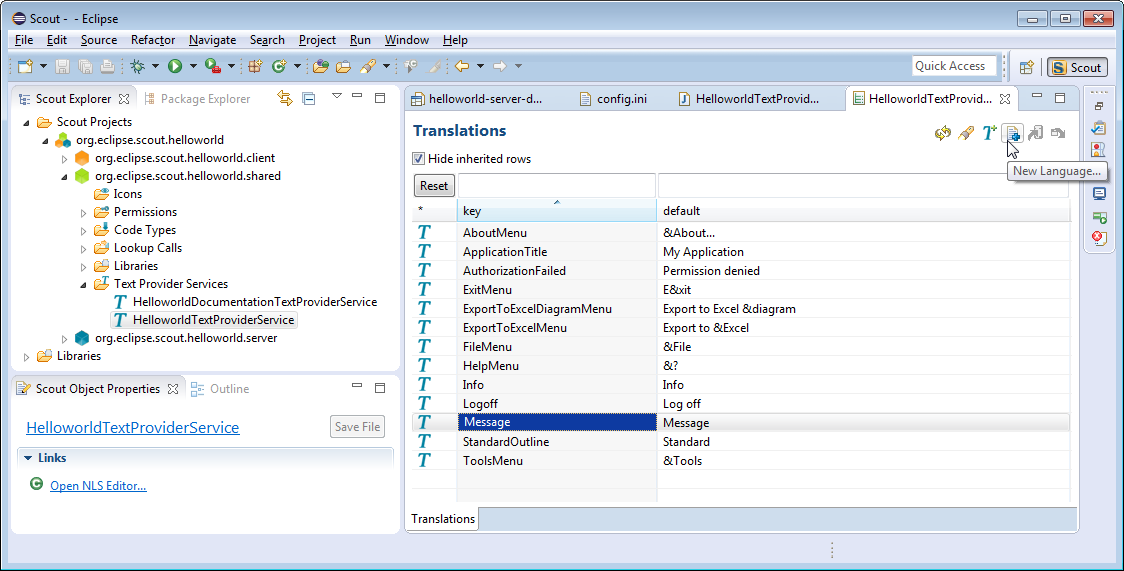
\includegraphics[width=14cm]{sdk_nls_editor.png} 
\caption{The NLS editor provided by the Scout SDK. This editor is opened via the \link{Open NLS Editor ...} in the Scout Object Properties of the \node{HelloworldTextProviderService}.
}
\index{NLS editor}
\figlabel{nls_editor}
\end{figure}

When we did add the \field{Message} to the desktop form of the ''Hello World'' application we had to enter a new translation entry for the label of the message field as shown in \figref{helloworld_stringfield}.
The individual translation entries are then stored in language specific text property files.
To modify translated texts we can use the NLS editor\footnote{
See \secref{nls_editor} for a detailed description of the NLS editor.
} 
provided by the Scout SDK as shown in \figref{nls_editor}.

To access the translated label field entry in the application, the Scout SDK generated the implementation of \java{getConfiguredLabel} using \java{TEXTS.get("Message")} as shown in \lstref{helloworld.mainbox}.
In the default Scout project setup, calling \java{TEXTS.get} uses the \java{DefaultTextProviderService} in the background.
This text provider service then defines the access path for the text property files to use for the translation.
To resolve the provided key, the user's locale settings are used to access the correct text property file.

% --------------------------------------------------------------------------- %
\section{The Server Part}
\seclabel{helloworld.server.background}

In this background section we take a closer look at Scout services and calling service methods remotely.
We will first discuss the setup of an ordinary Scout service.
Then, the additional components to call service methods remotely are considered.
To explain the concepts in a concrete context, we use the setup of the \java{DesktopService} of our ''Hello World'' example.

% ........................................................................... %
\subsection{Scout Services}

Scout services are OSGi services\footnote{
A good introduction to OSGi services is provided by Lars Vogel's tutorial: \url{http://www.vogella.com/articles/OSGiServices/article.html}.
}
which in turn are defined by standard Java classes or interfaces.
Scout is just adding a convenience layer to cover typical requirements in the context of client server applications. 
To support Scout developers as much as possible, the Scout SDK offers wizards that generate the necessary classes and interfaces and also take care of service registration.

\lstinputlisting[
  label=\lstlabel{helloworld.desktop_service},
  caption=The server service class \java{DesktopService}.,
  linerange={8-15},
  float
]
{../code/helloworld/org.eclipse.scout.helloworld.server/src/org/eclipse/scout/helloworld/server/services/DesktopService.java}

All Scout services need to extend Scout's \java{AbstractService} class and implement their own corresponding interface.
This also applies to the ''Hello World'' desktop service according to \lstref{helloworld.desktop_service}.
As shown in \figref{helloworld_load_servicemethod}, this service can be located in the Scout Explorer under the blue server node in the \folder{Services}.

Before Scout services can be accessed and used, they need to be explicitly registered as a service in the correct place.
For this registration mechanism, Scout is using Eclipse extension points and extensions\footnote{
A good introduction to Eclipse extensions and extension points is provided in the Eclipse wiki: \url{http://wiki.eclipse.org/FAQ_What_are_extensions_and_extension_points\%3F}.
}
which are conceptually similar to electrical outlets and plugs.
And in order to work, as in the case of outlets and plugs, the plug must fit to the outlet.
In our ''Hello World'' example, the extension (plug) is represented by class \java{DesktopService} and the service extension point (outlet) is named \java{org.eclipse.scout.service.services}.
What makes the desktop service fit to the service extension point is the fact that its interface \java{IDesktopService} extends Scout's \java{IService} interface.

\begin{figure}
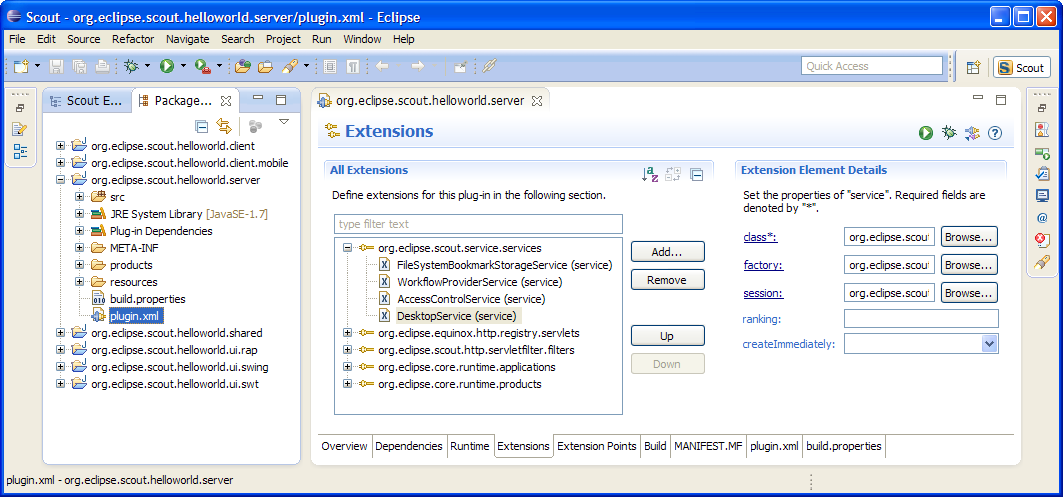
\includegraphics[width=14cm]{sdk_plugin_editor_desktopservice.png}
\caption{The Eclipse plugin editor for \java{plugin.xml} files.
In the tab \element{Extensions} the ''Hello World'' desktop service is registered under the extension point \java{org.eclipse.scout.service.services}.
}
\index{Eclipse plugin editor}
\figlabel{plugin_editor}
\end{figure}

\lstinputlisting[
  label=\lstlabel{helloworld.server_plugin_xml},
  caption=The registration of the \java{DesktopService} in the server's \java{plugin.xml} configuration file. The remaining content of the file has been omitted.,
  index={Plugin service registration},
  linerange={1-6,22-27,105-106},
  language=xml,
  float
]
{../code/helloworld/org.eclipse.scout.helloworld.server/plugin.xml}

The registration of the desktop service under the service extension point is then defined in the \filename{plugin.xml} file of the ''Hello World'' server plugin.
As shown in \figref{plugin_editor}, the \filename{plugin.xml} file is located in the root path of plugin \java{org.eclipse.scout.helloworld.server}.
To modify a \filename{plugin.xml}, you can either use the Eclipse plugin editor or your favorite text editor.
In \figref{plugin_editor}, the registration of the desktop service is shown in the \element{Extensions} tab of the plugin editor.
For the corresponding XML representation in the \filename{plugin.xml} file, see \lstref{helloworld.server_plugin_xml}.

% ........................................................................... %
\subsection{Scout Proxy Services}

In the ''Hello World'' application the \java{load} method of the desktop service is called remotely from the client.
But so far, we have only seen how the desktop service is implemented and registered in the server application.
To call server service methods remotely from Scout client applications, the Scout framework provides client proxy services and the service tunnel.
As the name implies, a client proxy service acts as a local proxy service (running in the Scout client application) of a server service (running remotely in the Scout server application).

\lstinputlisting[
  label=\lstlabel{helloworld.client_plugin_xml},
  caption=The registration of the \java{IDesktopService} proxy service in the client plugin of the ''Hello World'' application. This is the complete content of the client's \java{plugin.xml} file.,
  index={Plugin service registration},
  language=xml,
  float
]
{../code/helloworld/org.eclipse.scout.helloworld.client/plugin.xml}

Client proxy services are defined by a Java interface located in the shared plugin of the Scout application.
As shown in \lstref{helloworld.desktop_service} of the desktop service, this service interface is also implemented by the desktop service class in the server plugin.
Corresponding to the registration of the desktop service in the server plugin, client proxy services need to be registered in the client's \filename{plugin.xml} file.
The content of the ''Hello World'' client plugin configuration file is provided in \lstref{helloworld.client_plugin_xml}.
To create proxy services in Scout clients, the \java{ClientProxyServiceFactory} is used. 
This is also reflected in the extension defined in \lstref{helloworld.client_plugin_xml}.
Internally, this service factory then uses the service tunnel to create the local proxy services.

To call a remote service method from the Scout client application, we first need to obtain a reference to the proxy service.
Using the \java{SERVICES.getService} method with the interface \java{IDesktopService}, we can obtain such a reference as shown in \lstref{helloworld.viewhandler} for the view handler of the desktop form.
With this reference to the client's proxy service, calling methods remotely works as if the service would be running locally.
Connecting to the server, serializing the method call including parameters (and de serializing the return value) is handled transparently by Scout.

% --------------------------------------------------------------------------- %
\section{Add the Rayo Look and Feel}
\seclabel{helloworld.rayo.background}

Rayo has been designed in 2009 by BSI for its CRM\footnote{
Customer Relationship Management (CRM): \url{https://en.wikipedia.org/wiki/Customer_relationship_management}} 
application and contact center solution.
Since then, Rayo has been copied for Scout web applications and also adapted to work on touch/mobile devices.

The implementation of Rayo for desktop clients is based on the Java Synth look and feel\footnote{
Java Synth Look and Feel: \url{http://en.wikipedia.org/wiki/Synth_Look_and_Feel}
}.
However, in a few cases it was necessary to adjust some of the synth classes. 
In order to do this, the adapted classes are copied form the OpenJDK implementation\footnote{
OpenJDK is an open source implementation of the Java platform: \url{http://openjdk.java.net/}.
}
As OpenJDK is licenced under the GNU General Public Licence (GPL) with a linking exception it is not possible to distribute Rayo under the Eclipse Public Licence.
That is why Rayo is not initially contained in the Eclipse Scout package but needs to be downloaded from the Eclipse Marketplace.
Fortunately, there is still no restriction to use Rayo in commercial products.
The only remaining restriction applies to modifying Rayo for commercial products.
In this case you will be obliged to redistribute your modified version of Rayo under the same licence (GPL with classpath exception).

With Eclipse Scout 3.8 (Juno), the Scout framework also allows to build web clients based on Eclipse RAP.
Great care has been taken to ensure, that the look and feel for Scout web applications matches the look and feel of the desktop as closely as possible.
As RAP is already distributed under the EPL licence the Rayo for web apps is directly contained in the Scout package.
TODO: Describe what to change to use RAP default look and feel

A similar approach was chosen for Rayo on tablets and mobile devices that are supported with Eclipse Scout 3.9 (Kepler).
For such devices optimized components are used to take into account the smaller screens and the absence of a mouse (no context menus!)
But as far as possible, the Rayo look and feel also applies to touch devices.
TODO: Pointer to more info regarding mobile devices.

% --------------------------------------------------------------------------- %
\section{Exporting the Application}
\seclabel{helloworld_export_background}

In this background section we look at the content and organisation of the two WAR files generated by the Scout SDK \wizard{Export Scout Project}.
The first WAR file holds the Scout server including a landing page to download the Scout desktop client.
The desktop client is provided in the form of a standalone ZIP file.
In the second WAR file, the Ajax server based on Eclipse RAP is contained.
This Ajax server provides the URLs that can be accessed by web browsers running on desktop computers or tablet and mobile devices.

\begin{figure}
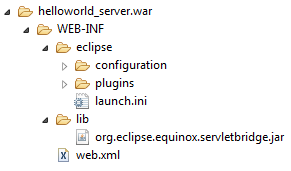
\includegraphics[height=4cm]{helloworld_server_war.png} \hspace{5mm}
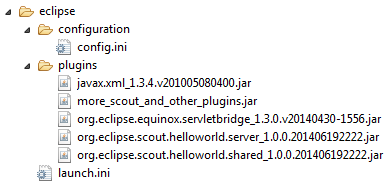
\includegraphics[height=4cm]{helloworld_server_war_eclipse.png}
\caption{The organisation of the ''Hello World'' server WAR file.
The right side reveals the location of the \java{config.ini} file and the application's plugin files} 
\figlabel{helloworld_server_war}
\end{figure}

The content and its organisation of the exported WAR files was not specifically designed for Scout applications. 
Rather, it is defined according to server-side Equinox\footnote{
See \appref{osgi_basics} for more information regarding server-side Equinox.
},
the typical setup for running Eclipse based server applications on a web server.
Using file \filename{helloworld_server.war} as a concrete example, we will first describe the general organisation of the WAR file.
Then, we introduce individual artefacts of interest that are contained in this WAR file.

The explicit organisation of the server WAR file is shown in \figref{helloworld_server_war}.
From the left hand side of the figure we can see that on the top level only folder \filename{WEB-INF} exists in the WAR file.
This folder contains all files and directories that are private to the web application.
Inside, the web deployment descriptor file \filename{web.xml} as well as the directories \filename{lib} and \filename{eclipse} are located.
While the \filename{web.xml} file and directory \filename{lib} are standard for servlet based based applications\footnote{
See \appref{javaee_basics} for more information regarding servlets.
},
directory \filename{eclipse} contains all necessary artefacts for servlet based Eclipse applications\footnote{
See \appref{osgi_basics} for more information regarding server-side Eclipse applications (server-side Equinox). 
}.
Such as Eclipse Scout server applications.

On the right hand side of \figref{helloworld_server_war} the eclipse specific content of the WAR file is shown.
From top to bottom we find the configuration file \filename{config.ini} introduced in \secref{config_ini}.
In folder \filename{plugins} the necessary plugins that constitute the eclipse application are located where the plugins are available in the form of JAR files\footnote{
JAR files contain a set of Java classes and associated resources. \url{http://en.wikipedia.org/wiki/JAR_\%28file_format\%29}.
}.
This includes plugins for servlet management, the eclipse platform including the servlet bridge, the scout framework parts and of course our ''Hello World'' server and shared plugin.
These ''Hello World'' jar files exactly match with the plugin projects discussed in \secref{create_project_simple_background}.

\begin{figure}
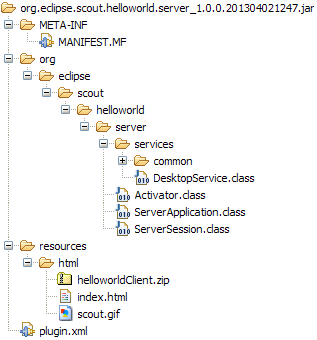
\includegraphics[height=9cm]{helloworld_server_war_plugin.png} 
\caption{The content of the ''Hello World'' server plugin contained in the \java{helloworld\_server.war} file.
The necessary files for the download page including the zipped client application are in the \java{resources/html} directory.} 
\figlabel{helloworld_server_plugin}
\end{figure}

\lstinputlisting[
  label=\lstlabel{helloworld.server_plugin_xml.resourceservlet},
  caption=The configuration of the server's resource servlet in the \java{plugin.xml} configuration file. The remaining content of the file has been omitted.,
  linerange={1-3,28-30,51-62,104-106},
  language=xml,
  float
]
{../code/helloworld/org.eclipse.scout.helloworld.server/plugin.xml}

In \figref{helloworld_server_plugin} some of the content of the ''Hello World'' server plugin is shown.
The first thing to note is that the plugin file conforms to the JAR file format including a \filename{META-INF/MANIFEST.MF} file and the directory tree containing the Java class files, as the \filename{DesktopService.class} implemented in \secref{helloworld.server} of the ''Hello World'' tutorial.
In folder \filename{resources/html} the necessary files for the download page shown in \figref{helloworld_running_download} including the zipped desktop client are contained.
To access this download page the Scout server's resource servlet \java{ResourceServlet} is responsible.
It is registered under the servlet registry as shown in \lstref{helloworld.server_plugin_xml.resourceservlet}.
With setting "/" of the \java{alias} parameter the download page becomes available under the root path of the Scout server application.
For the mapping to the contents \filename{resources/html} the parameter \java{bundle-path} is used.

\begin{figure}
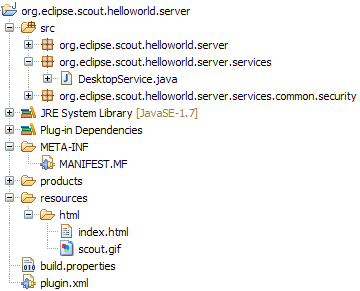
\includegraphics[height=8cm]{helloworld_server_plugin.png} 
\caption{The ''Hello World'' server plugin shown in the Eclipse package explorer.
The files for the download page are located under \java{resources/html}.} 
\figlabel{helloworld_server_explorer}
\end{figure}

Revisiting the ''Hello World'' server plugin project in the Eclipse package explorer as shown in \figref{helloworld_server_explorer}, we can see how the plugin project elements are transformed and copied into the JAR file.
Examples files are \filename{plugin.xml} and \filename{MANIFEST.MF} as well as static HTML content of the download page (files \filename{index.html} and \filename{scout.gif}).
The zipped client is missing of course.
It is assembled, zipped and added into the Scout server JAR file by the \wizard{Export Scout Project} of the Scout SDK.
In case you need to change/brand/amend the download page for the desktop client, you have now learned where to add and change the corresponding HTML files.

% --------------------------------------------------------------------------- %
\section{Deploying to Tomcat}
\seclabel{helloworld.tomcat.background}

In this section we will discuss two common pitfalls when working with the Scout IDE and Tomcat.
The symptoms linked to these problems are Scout server applications that are not starting or Scout applications that fail to properly update.

In usual culprit behind Scout server applications that fail to start is a blocked port 8080.
This setting can be created when we try to run both the Jetty web server inside the Scout SDK and the local Tomcat instance.
In consequence, either Jetty or Tomcat is not able to bind to port 8080 at startup which makes it impossible for a client to connect to the right server.
To avoid such conflicts, make sure that you always stop the Scout server application in the Scout SDK (effectively killing Jetty) before you restart your Tomcat server.
Alternatively, you can assign two different ports to your Jetty webserver and your Tomcat webserver.

To modify Jetty's port number in the Scout SDK you have to update the corresponding properties in the \filename{config.ini} files of the development products of your Scout server application and all client applications.
In the Scout server's \filename{config.ini} file the property is named \java{org.eclipse.equinox.http.jetty.http.port}, in the client \filename{config.ini} files the relevant property is called \java{server.url}.
To change the port number to 8081 for the ''Hello World'' example in the Scout SDK you could use the following lines in the individual \filename{config.ini} files.

\begin{tabular}{ll}
 Scout Server         & org.eclipse.equinox.http.jetty.http.port=8081              \\
 Scout Desktop Client & server.url=http://localhost:8081/helloworld\_server/process \\
 Scout Ajax Server    & server.url=http://localhost:8081/helloworld\_server/ajax
\end{tabular}

The second pitfall is connected to a web application that seems to refuse to update to the content of a freshly generated WAR file.
At times it seems that your changes to a deployed WAR file do not find their way to the application actually running. 
In many cases this is caused by a cached instance of the previous version of your application located in Tomcat's working directory.
To save yourself much frustration, it often helps just to clear Tomcat's working directory and restart Tomcat.
For this, you may follow the following procedure.

\begin{enumerate}
  \item Stop the Tomcat web server
  \item Go to folder \filename{work/Catalina/localhost}
  \item Verify that you are not in Tomcat's \filename{webapps} folder
  \item Delete all files and directories in folder \filename{work/Catalina/localhost}
  \item Start the Tomcat web server
\end{enumerate}

How you start and stop Tomcat depends on the platform you are running it. 
If you have installed Tomcat on a Windows box according to \appref{install_tomcat} it will be running as a service.
This means that to stop the Tomcat web server you need to stop the corresponding Windows service.
For starting and stopping Tomcat on Mac/Linux/Unix systems, you can use the command line script files \filename{startup.sh} and \filename{shutdown.sh} located in Tomcat's subdirectory \filename{bin}.

For those interested in more advanced aspects of Apache Tomcat we recommend the article ''More about the Cat'' by Chua Hock-Chuan\footnote{
More about the Cat: \url{http://www.ntu.edu.sg/home/ehchua/programming/howto/Tomcat_More.html}.
}.

% --------------------------------------------------------------------------- %

\ifx\wholebook\relax\else
   \begin{thebibliography}{99}
  \addcontentsline{toc}{chapter}{Bibliography}
  
  % add/insert books in alphabetical order of 1st author
  
  \bibitem{batessierra05}
    \textit{Bert Bates, Kathy Sierra},
	\textbf{Head First Java} 2nd edition, 
	O'Reilly Media, 2005.

  \bibitem{bloch08} 
    \textit{Joshua Bloch},
    \textbf{Effective Java} 2nd edition, 
	Addison-Wesley, 2008.
	
  \bibitem{eckel06}
    \textit{Bruce Eckel},
	\textbf{Thinking in Java} 4th edition, 
	Prentice Hall International, 2006.

\end{thebibliography}

   \end{document}
\fi

% =========================================================================== %
